% !TEX encoding = UTF-8 Unicode
% !TEX root = thesis.tex

\chapter{Measuring Total Body Motion Capture}
\label{chapter:totalcapture}



\section{Introduction}
Social communication is a key function of human motion \cite{Birdwhistell70}. We communicate tremendous amounts of information with the subtlest movements. Between a group of interacting individuals, gestures such as a gentle shrug of the shoulders, a quick turn of the head, or an uneasy shifting of weight from foot to foot, all transmit critical information about the attention, emotion, and intention to observers. Notably, these social signals are usually transmitted by the organized motion of the whole body: with facial expressions, hand gestures, and body posture. These rich signals layer upon goal-directed activity in constructing the behavior of humans, and are therefore crucial for the machine perception of human activity. 

However, there are no existing systems that can track, without markers, the human body, face, and hands simultaneously. Current markerless motion capture systems focus at a particular scale or on a particular part. Each area has its own preferred capture configuration: (1) torso and limb motions are captured in a sufficiently large working volume where people can freely move~\cite{deAguiar-2008, Gall-09, Stoll-11, Elhayek-15}; (2) facial motion is captured at close range, mostly frontal, and assuming little global head motion~\cite{Beeler:SIGGRAPH2010,ghosh2011multiview, Beeler:SIGGRAPH2011, bradley2010high, valgaerts2012lightweight}; (3) finger motion is also captured at very close distances from hands, where the hand regions are dominant in the sensor measurements~\cite{Oikonomidis-12, Tompson-14a, Sridha-15, Tzionas-16}. These configurations make it difficult to concurrently analyze the full spectrum of social signalling.

% % The following paragraph has nicer sentences than above:

%In this paper, we present an approach to capture the motion of the principal body parts for multiple interacting people (see Fig.~\ref{fig:teaser2}). The fundamental difficulty of such capture is caused by the scale differences of each part. For example, the torso and limbs are relatively large and necessitate coverage over a sufficiently large working volume, while fingers and faces, due to their smaller feature size, require close distance capture with high resolution and frontal imaging. With off-the-shelf cameras, the resolution for face and hand parts will be limited in a room-scale, multi-person capture setup. 

To overcome this sensing challenge, we present a novel generative body deformation model that has the ability to express the motion of each principal body part. In particular, we describe a procedure to build an initial body model, named ``Frank", by seamlessly consolidating available part template models~\cite{Loper2015,cao2014facewarehouse} into a single skeleton hierarchy. To fit this model to data, we leverage keypoint detection (e.g., faces~\cite{Torre15}, bodies~\cite{Wei2016,cao2016realtime,Newell-16}, and hands~\cite{simon2017hand}) in multiple views to obtain 3D keypoints which are robust to multiple people and object interactions. We fit the ``Frank'' model to a capture of 70 people, and learn a new deformation model, named ``Adam", capable of additionally capturing variations of hair and clothing with a simplified parameterization. We present a method to capture the total body motion of multiple people with the 3D deformable model. Finally, we demonstrate the performance of our method on various sequences of social behavior and person-object interactions, where the combination of face, limb, and finger motion emerges naturally.

\section{Related Work}

Marker-based motion capture systems that track retro-reflective markers~\cite{VICON, woltring1973new} are the most widely used method to capture human body motion. However, in addition to a laborious process of attaching markers on subjects, these methods still suffer from major limitations including: (1) a necessity of sparsity in marker density for reliable tracking, which limits the spatial resolution of motion measurements~\cite{park2006capturing}; (2) a limitation in automatically handling occluded markers which requires expensive manual clean-up; and (3) markers on the faces, bodies, and hands hinder participants from engaging in natural social interaction. Due to these limitations, capturing the total body motion of interacting people is still a challenging problem even in state-of-the-art motion capture systems~\cite{VICON}. 

Markerless motion capture methods have been explored over the past two decades to achieve the same goal of motion capture systems, but they tend to implicitly admit that their performance is inferior to their marker-based counterpart, advocating their ``markerless'' nature as the major advantage. Most markerless motion capture methods largely focus on the motion of the torso and limbs. The standard pipeline is based on a multiview camera setup and tracking with a 3D template model~\cite{Liu-2013, Gavrila-96, Cheung-05, Bregler-04, Kehl-06, Corazza-10, Vlasic-08, Brox-10, Stoll-11, deAguiar-2008, Elhayek-15}. In this approach, motion capture is performed by aligning a 3D template model to the measurements, which can include colors, textures, silhouettes, point clouds, and keypoints. Recent methods exploit a generative deformable body model~\cite{anguelov2005scape, Loper2015, pons2015dyna} to express both shape and body variations of humans. Since these body models often assume minimum clothing for subjects, explicit modeling for clothing is needed to capture clothed subjects~\cite{zhang2017detailed, pons2017clothcap}. Recent advances in 2D keypoint detection~\cite{ Newell-16, cao2016realtime, Wei2016} make it possible to reliably reconstruct 3D keypoints in a multiview setup, where a 3D model can be fitted~\cite{Elhayek-15, Joo-15, joo2017panoptic}. A specific strength of learning-based detectors is that they can provide a ``guess"  for occluded parts, based on the spatial human body configurations learned from a large-scale 2D pose dataset. Note that we differentiate markerless motion capture approaches, producing motion parameters as output, from multiview performance capture approaches~\cite{Vlasic-2009, Furukawa-2008} which aim to obtain detailed surface shapes by free-form mesh deformations. With the introduction of commodity depth sensors, single-view depth-based body motion capture also became a popular direction~\cite{Baak-13, Shotton2011}. More recently, a collection of approaches aims to reconstruct 3D skeletons directly from monocular images, either by fitting 2D keypoint detections with a prior on human pose~\cite{Zhou2015,Bogo2016} or getting even closer to direct regression methods~\cite{Zhou2016,Mehta2017,tome2017lifting}.

In all earlier work, face and hand motion captures are often considered as separate research domains.  Facial scanning and performance capture has been greatly advanced over the last decade. There exist multiview methods showing excellent performance on high-quality facial scanning~\cite{Beeler:SIGGRAPH2010,ghosh2011multiview} and facial motion capture~\cite{Beeler:SIGGRAPH2011, bradley2010high, valgaerts2012lightweight}. Recently, lightweight systems based on a single camera show compelling performance by leveraging a morphable 3D face model on 2D measurements~\cite{garrido-tog-2013, Torre15, li2013realtime, thies2016face2face, cao2014facewarehouse, cao2015real, wu2016anatomically}. Most of these methods are based on a deformable 3D face rig such as the method of Cao et al. \cite{cao2014facewarehouse}. Hand motion capture is mostly led by single depth-sensor based methods~\cite{Oikonomidis-12, Tang-14, Tompson-14a, Keskin-12,Xu-13,Sun-15,Wan-16, Sridhar-13, Sharp-15, Sridha-15, Tzionas-16, Ye-16}, with few exceptions based on multi-view systems~\cite{Ballan-12, Sridhar-13, MANO:SIGGRAPHASIA:2017}. Recently, 2D hand keypoint detection and the use of it to obtain 3D hand keypoints in a multiview setup are introduced by Simon et al.~\cite{simon2017hand}. Notably, a generative 3D model that can express body and hands was also introduced by Romero et al.~\cite{MANO:SIGGRAPHASIA:2017}. 

In contrast, this paper presents the first approach for ``total'' markerless motion capture of multiple interacting people, producing a parameterized representation that jointly captures the time-varying body pose, hand pose, and facial expressions of each of the interacting participants. %To accomplish this, we use a calibrated multiview camera system and unify existing part models for the body, hands, and face into a single skeleton hierarchy and model that we call ``Adam'', which can more easily be fit to people engaging in natural social interactions.

% !TEX encoding = UTF-8 Unicode
% !TEX root = ../thesis.tex


%
%\section{Overview}
%In this paper, we present two human body prior models for total body motion capture. 
%% The major reason of presenting two models is the fact that we need a way to accurately reconstruct total body shape and motion first in order to build a new model learnt from the data, which is a chicken and egg problem.  
%%Instead of building the desired body model from the scratch,
%We first present the ``Frankenstein model" to consolidate existing high-quality part models (face, body, and hands) into a single skeleton hierarchy. Capturing shape and motion of the total body is then possible by fitting the Frankenstein model to 3D sensor measurements, including 3D keypoints and 3D point clouds. We find that total motion capture with the Frankenstein model already produces compelling results, as shown in the accompanying video. However, there are several aspects that need improvement: (1) the model only produces shapes without hair and clothing; (2) model optimization is complex, and requires additional optimization parameters to keep the parts connected without artifacts, making implementation complicated; and (3) the definition of joints for the 2D detectors is different from the actual location of the joints in the 3D skeleton, resulting in a nonzero cost function even for the correct pose.
%
%To this end, we present a model, named ``Adam", aiming to capture total body motion with a simpler parameterization. The model is built from the reconstruction data leveraged by the Frankenstein model for various motions of 70 subjects. Since the reconstruction data has diversity in clothings and hairs, the learned linear subspace model of Adam has a degree of expressive power for hairs and clothing. 
%
%Finally, we evaluate our method on various challenging sequences captured in the CMU Panoptic Studio~\cite{Joo-15}.

%
%\subsection{Discussion}
%\label{Franken:discussion}
%We find that total motion capture with the Frankenstein model already produces compelling results, as shown in the accompanying video. However, there are several aspects which need improvements: 1) the model only produces shapes without hairs and clothing, very different from the natural interactions we aim to capture; 2) model optimization is complex, and requires additional optimization parameters to keep the parts connected without artifacts, making implementation complicated, and 3) the definition of joints for the 2D detectors is different from the actual location of the joints in the 3D skeleton, resulting in a nonzero cost function even for the correct pose.

%

% \begin{figure}[t]
% 	%	\includegraphics[width=0.49\columnwidth]{fig/smpl_parts_aligned_3}
% 	%	\includegraphics[width=0.49\columnwidth]{fig/totalmesh_3}
% 	%\includegraphics[width=\columnwidth]{totalmodelbuilding4}
% 	\includegraphics[width=0.9\columnwidth]{Partmodels_180326.pdf}
% 	\caption{Part models and the Frank model. (a) The body model~\cite{Loper2015}; (b) the face model~\cite{cao2014facewarehouse}; and (c) a hand rig. In (a-c), the red dots have corresponding 3D keypoints reconstructed by detectors.} %(d) Aligned face and hand models (gray meshes) to the body model (the blue wireframe mesh); and (e) the seamless Frank model.}
% 	\label{fig:frankenstein_part_aligned}
% 	%	\label{fig:frankenstein_mesh}
% 	% Yaser: (d) and (e) as a separate figure
% \end{figure}

\begin{figure}[t]
	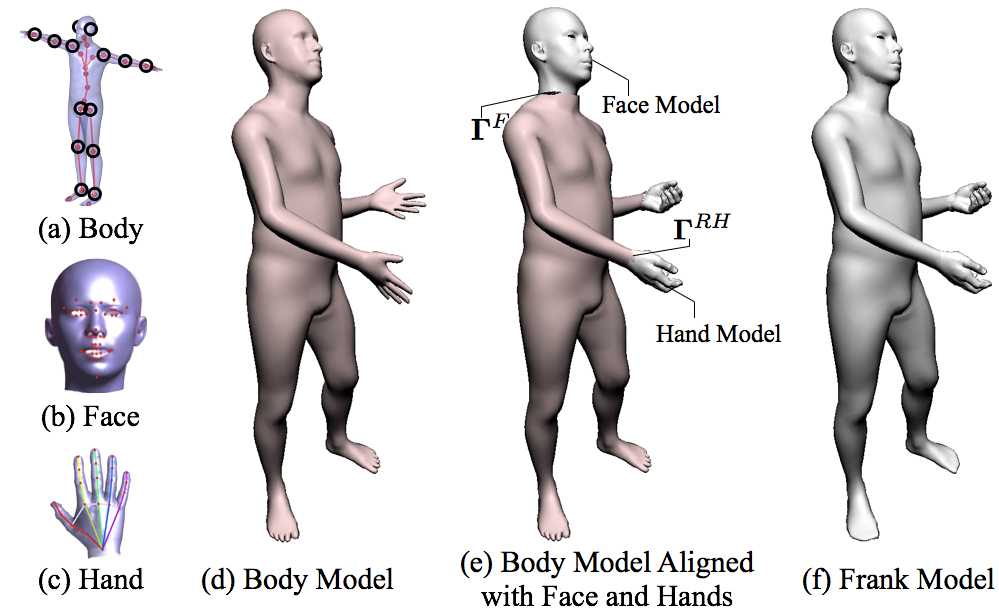
\includegraphics[trim={1cm 0 0 0 }, width=\columnwidth]{tbc_figures/building_frank_3}
	\caption{Part models and the Frank model. (a) The body model~\cite{Loper2015}; (b) the face model~\cite{cao2014facewarehouse}; and (c) a hand rig. In (a-c), the red dots have corresponding 3D keypoints reconstructed by detectors; (d) Body only model; (e) Face and hand models substitute the corresponding parts of the body model. Alignments are ensured by  $\bm{\Gamma}$s; and (f) The blending matrix $\mathbf{C}$ is applied to produce a seamless mesh.} %(d) Aligned face and hand models (gray meshes) to the body model (the blue wireframe mesh); and (e) the seamless Frank model.}
	\label{fig:frankenstein_part_aligned}
	%	\label{fig:frankenstein_mesh}
	% Yaser: (d) and (e) as a separate figure
\end{figure}

\section{Frank Model}

The motivation for building the Frank\footnote{Frank is an homage to a certain \emph{Modern Prometheus}.} body model is to leverage existing part models: SMPL~\cite{Loper2015} for the body, FaceWarehouse~\cite{cao2014facewarehouse} for the face, and an artist-defined hand rig (shown in Fig.~\ref{fig:frankenstein_part_aligned}). Each of these capture shape and motion details at an appropriate scale for the corresponding part.
%Thus, we have a coarser mesh for the body torso and limbs, and more detailed meshes for the face and the hands. 
This choice is not driven merely by the free availability of the component models: note that due to the trade-off between image resolution and field of view of today's 3D scanning systems, scans used to build detailed face models will generally be captured using a different system than that used for the rest of the body.
%In the near future, it is therefore likely that full-body models will be constructed by merging more detailed component models. 
For our model, we merge all transform bones into a single skeletal hierarchy but keep the native parameterization of each component part to express identity and motion variations. As the final output, the Frank model produces motion parameters capturing the total body motion of humans, and generates a seamless mesh by blending the vertices of the component meshes. 

\subsection{Stitching Part Models}

The Frank model $M^U$ is parameterized by motion parameters $\boldsymbol{\theta}^U$, shape (or identity) parameters $\boldsymbol{\phi}^U$, and a global translation parameter $\mathbf{t}^U$,
\begin{align}
\mathbf{V}^U = M^U (\boldsymbol{\theta}^U, \boldsymbol{\phi}^U, \mathbf{t}^U ),
\end{align}
where $\mathbf{V}^U$ is a seamless mesh expressing the motion and shape of the target subject.  The motion and shape parameters of the model are a union of the part models' parameters:
\begin{align}
\boldsymbol{\theta}^U = \{ \boldsymbol{\theta}^B, \boldsymbol{\theta}^F, \boldsymbol{\theta}^{LH}, \boldsymbol{\theta}^{RH}  \}, \\
\boldsymbol{\phi}^U = \{ \boldsymbol{\phi}^B, \boldsymbol{\phi}^F, \boldsymbol{\phi}^{LH},  \boldsymbol{\phi}^{RH}  \},
%\mathbf{t}^U_t = \{ \mathbf{t}^B_t, \mathbf{t}^F_t, \mathbf{t}^{LH}_t, \mathbf{t}^{RH}_t  \}
\end{align}
where the superscripts represent each part model: $B$~for the body model, $F$ for the face model, $LH$ for the left hand model, and $RH$ for the right hand model. Each of the component part models maps from a subset of the above parameters to a set of vertices, respectively, $\mathbf{V}^B \,{\in}\, \mathds{R}^{N^B{\times}3}$, $\mathbf{V}^F \,{\in}\, \mathds{R}^{N^F{\times}3}$, $\mathbf{V}^{LH} \,{\in}\, \mathds{R}^{N^H{\times}3}$, and $\mathbf{V}^{RH} \,{\in}\, \mathds{R}^{N^H{\times}3}$, where the number of vertices of each mesh part is $N^B{=}6890$, $N^F{=}11510$, and $N^H{=}2068$. The final mesh of the Frank model, $\mathbf{V}^U {\in} \mathds{R}^{N^U{\times}3}$, is defined by linearly blending them with a matrix $\mathbf{C} \in \mathds{R}^{N^U\times(N^B{+}N^F{+}2N^H)}$: 
\begin{align}
\mathbf{V}^U = \mathbf{C} 
\left[
\begin{array}{c}
\left({\mathbf{V}^B}\right)^T
\left({\mathbf{V}^F}\right)^T
\left({\mathbf{V}^{LH}}\right)^T
\left({\mathbf{V}^{RH}}\right)^T
\end{array} 
\right]^T,
\end{align}
where $T$ denotes the transpose of a matrix. Note that $\mathbf{V}^U$ has fewer vertices than the sum of part models because there are redundant parts in the body model (e.g., face and hands of the body model). In particular, our final mesh has $N^U{=}18540$ vertices. 
%If we separate Fig. 2. <--- look at Yaser's notes here
Fig.~\ref{fig:frankenstein_part_aligned} (e) shows the part models that are aligned, and (f) shows the final mesh topology of the Frank model after applying the the blending matrix $\mathbf{C}$ at the mean shape in the rest pose. 
%We define the mesh topology (vertex locations and faces) such that the boundary regions among parts are as seamless as possible. 
The blending matrix $\mathbf{C}$ is a very sparse matrix; most rows have a single column set to one with zeros elsewhere and simply copy the vertex locations from the corresponding part models with minimal interpolation at the seams.

%
%\begin{figure}[t]
%	\includegraphics[width=\columnwidth]{fig/C_mat_vis_}
%	\caption{C matrix to fuse output of part models. Showing block kind of structure of the matrix}
%	\label{fig:Total body fusion  matrix}
%\end{figure}
In the Frank model, all parts are rigidly linked by a single skeletal hierarchy, which is crucial as an output of motion capture. This unification is achieved by substituting the hands and face branches of the SMPL body skeleton with the corresponding skeletal hierarchies of the detailed part models. All parameters of the Frank model are jointly optimized for motion tracking and identity fitting. The parameterization of each of the part models is detailed in the following sections.
%, and then the joint optimization method for total body motion tracking with Frankenstein model is presented. 


%\begin{figure}[t]
%	\centering
%	%\includegraphics[width=\linewidth,clip=true,trim=60pt 0pt 0pt 0pt]{figures/fullbody/smpl_correspond}
%	\includegraphics[width=\linewidth]{figures/fullbody/smpl_correspond}
%	\caption{(a)~SMPL model~\cite{Loper2015}, template shapes (male and female) and first two basis vectors of shape variation. (b)~SMPL model joint hierarchy. Joints or vertices with a direct correspondence to a detected point are circled. (c)~2D detections corresponding to the outlined joints.\label{fig:smpl_correspond}} 
%\end{figure}



\subsection{Body Model}

For the body, we use the SMPL model~\cite{Loper2015} with minor modifications. 
%The SMPL model is a principal component analysis (PCA) based model of body shape that is deformed via linear blend skinning and pose-dependent corrective blendshapes. 
In this section, we summarize the salient aspects of the model in our notation. The body model, $M^B$, is defined as follows,
\begin{align}
\mathbf{V}^B = M^B (\boldsymbol{\theta}^B, \boldsymbol{\phi}^B, \boldsymbol{t}^B ),
\end{align}
with $\mathbf{V}^B = \{ \mathbf{v}^B_i\}_{i=1}^{N^B}$. 
The model uses a template mesh of $N^B{=}6890$ vertices, where we denote the $i$-th vertex as $\mathbf{v}^B_i\in\mathds{R}^3$. 
% The vertices of this template mesh are first displaced by a set of blendshapes describing the {\em identity} or body shape, yielding mesh vertices $\hat{\mathbf{v}}^B_i$ in the rest shape,
% \begin{align}
% \hat{\mathbf{v}}^B_i = \mathbf{v}^{B0}_i + \sum_{k=1}^{K_b} \mathbf{b}^k_{i} \phi^B_k,
% \label{eq:smpl_shape_coeffs}
% \end{align}
% where $\mathbf{b}^k_{i}\in\mathds{R}^3$ is the $i$-th vertex of the $k$-th blendshape, $\phi^B_k$ is the $k$-th shape coefficients of $\mathbf{\phi^B}\in\mathds{R}^{K_b}$, $K_b=10$ is the number of identity body shape coefficients, and $\mathbf{v}^{B0}_i$ is the $i$-th vertex of the mean shape.
% Given the vertices in the rest pose, the posed mesh vertices are obtained by linear blend skinning using transformation matrices $\mathbf{T}_j\in\mathds{R}^{4\times 4}$ for each of the $J$ joints,
% \begin{align}
% \mathbf{v}_i^B= \mathbf{I}_{3\times 4} \cdot \sum_{j=1}^{J^B} w_{i,j}\mathbf{T}^B_j (\theta^B) \begin{pmatrix} \hat{\mathbf{v}}^B_i \\ 1 \end{pmatrix},
% \label{eq:full_lbs_pose}
% \end{align}
% where the transformation matrices $\mathbf{T}_j$ encode the transform for each joint $j$ from the rest pose to the posed mesh in world coordinates, which is constructed by following skeleton hierarchy from the root joint. The $j$-th pose parameter $\boldsymbol{\theta}_j$ is the angle-axis representation of the relative rotation of joint $j$ with respect to its parent joints. $w_{i,j}$ is the weight with which transform $\mathbf{T}_j$ affects vertex $i$, with $\sum_{j=1}^Jw_{i,j}{=}1$ and $\mathbf{I}_{3\times 4}$ is the $3{\times} 4$ truncated identity matrix to transform from homogenous coordinates to a $3$ dimensional vector. We use $J^B{=}21$ with $\theta^B \,{\in}\, \mathds{R}^{21{\times}3}$, ignoring the last joint of each hand compared to the original SMPL model. For simplicity, we do not use the pose-dependent blendshapes during fitting.
The vertices of this template mesh are first displaced by a set of blendshapes describing the {\em identity} or body shape. Given the vertices in the rest pose, the posed mesh vertices are obtained by linear blend skinning (LBS) using transformation matrices $\mathbf{T}^B_j\in \textrm{SE(3)}$ for each of the $J$ joints,
\begin{align}
\mathbf{v}_i^B= \mathbf{I}_{3\times 4} \cdot \sum_{j=1}^{J^B} w^B_{i,j}\mathbf{T}^B_j\begin{pmatrix} \mathbf{v}^{B0}_i + \sum_{k=1}^{K_b} \mathbf{b}^k_{i} \phi^B_k \\ 1 \end{pmatrix},
\label{eq:full_lbs_pose}
\end{align}
where $\mathbf{b}^k_{i}\in\mathds{R}^3$ is the $i$-th vertex of the $k$-th blendshape, $\phi^B_k$ is the $k$-th shape coefficient in $\boldsymbol{\phi}^B\in\mathds{R}^{K_b}$ with $K_b{=}10$ the number of identity body shape coefficients, and $\mathbf{v}^{B0}_i$ is the $i$-th vertex of the mean shape. The transformation matrices $\mathbf{T}^B_j$ encode the transform for each joint $j$ from the rest pose to the posed mesh in world coordinates, which is constructed by traversing the skeleton hierarchy from the root joint with pose parameter $\boldsymbol{\theta}^B$ (see~\cite{Loper2015}). The $j$-th pose parameter $\theta^B_j$ is the angle-axis representation of the relative rotation of joint $j$ with respect to its parent joints. $w^B_{i,j}$ is the weight with which transform $\mathbf{T}^B_j$ affects vertex $i$, with $\sum_{j=1}^{J^B}w^B_{i,j}{=}1$ and $\mathbf{I}_{3\times 4}$ is the $3{\times} 4$ truncated identity matrix to transform from homogeneous coordinates to a $3$ dimensional vector. We use $J^B{=}21$ with $\boldsymbol{\theta}^B \,{\in}\, \mathds{R}^{21{\times}3}$, ignoring the last joint of each hand of the SMPL model. For simplicity, we do not use the pose-dependent blendshapes\footnote{For our target sequences, the modeling error between the SMPL model~\cite{Loper2015} and the 3D surface measurements is dominated by clothing artifacts, which the pose-blendshapes were not trained on.}.
%While the original SMPL model has $J^B{=}24$ with $23$ joints and an additional root transform to orient the body in world-space coordinates, we omit the last joint of each hand, and use $J^B{=}21$ with $\theta^B \,{\in}\, \mathds{R}^{21{\times}3}$. For simplicity, we do not use the pose-dependent blendshapes during fitting; this results in faster optimization runtimes and a sparser Jacobian matrix during the minimization.
% Additionally, we use only the male model as we will deform the surface to match each person's surface.

% The transformation matrices $\mathbf{T}_j$ encode the transform for each joint $j$ from the rest pose to the posed mesh in world coordinates, and are a function of the joint angles $\boldsymbol{\theta}\in\mathds{R}^{3\times J}$ (including the world-space orientation of the body) and the world-space translation $t \in\mathds{R}^3$. Each column $\boldsymbol{\theta}_j$ is the angle-axis representation of the relative rotation of joint $j$ with respect to its parent joint. A key characteristic of the SMPL model is that these transformations also depend on the shape coefficients $\mathbf{a}$; we refer the reader to~\cite{Loper2015} for details on the construction of these matrices. Let us call $\mathbf{V}_b{=}[\mathbf{v}_1 \dots \mathbf{v}_V]\in\mathds{R}^{3\times V}$ the full set of posed vertices in world coordinates. We can then compose the action of Eq.~\eqref{eq:smpl_shape_coeffs} and Eq.~\eqref{eq:full_lbs_pose} into a function that transforms from the set of body parameters (body shape $\mathbf{a}$, body pose $\boldsymbol{\theta}$, and translation $\mathbf{t}$) to the posed vertices of the body mesh in world coordinates,
%\begin{align}
%\mathbf{V}_b = b( \mathbf{a}, \boldsymbol{\theta}, \mathbf{t} ).
%\end{align}
%Fig.~\ref{fig:smpl_correspond}a shows the vertices of the SMPL model in its rest pose, color coded to illustrate the region of influence of each bone. Each color corresponds to a different bone, and the smooth blending between colors reflects the changing relative weights of each of the bones influencing a single vertex. Fig.~\ref{fig:smpl_correspond}b shows the full joint hierarchy, which at $23$ joints is more complex than the subset of joints detected (Fig.~\ref{fig:smpl_correspond}c) and triangulated (Fig.~\ref{fig:smpl_correspond}d) by the method of Sect.~\ref{sect:markerless_mocap}. Note that the detected points do not cover all degrees of freedom captured by the SMPL model, particularly details about body shape as well as the orientation of certain limbs, notably the forearms, head, and feet.

\subsection{Face Model}
\label{subsection:face}
As a face model, we build a generative PCA model from the FaceWarehouse dataset~\cite{cao2014facewarehouse}. Specifically, the face part model, $M^F$, is defined as follows,
\begin{align}
\mathbf{V}^F = M^F (\boldsymbol{\theta}^F, \boldsymbol{\phi}^F, \mathbf{T}^F ),
\end{align}
with $\mathbf{V}^F = \{ \mathbf{v}^F_i\}_{i=1}^{N^F}$, where the $i$-th vertex is $\mathbf{v}^F_i\in\mathds{R}^3$, and $N^F{=}11510$. The vertices are represented by combining shape and expression subspaces:
%The model uses a template mesh of $N^F{=}11510$ vertices, where we denote the $i$-th vertex as $\mathbf{v}^F_i\in\mathds{R}^3$. We decompose the shapes in the dataset into two linear subspaces, one corresponding to identity and one corresponding to expression variations. The $i$-th face vertex is represented by the linear combination of the subspaces:
\begin{align}
\hat{\mathbf{v}}_i^F = \mathbf{v}^{F0}_i + \sum_{k=1}^{K_{f}} \mathbf{f}^k_{i} \phi^F_k  + \sum_{s=1}^{K_{e}} \mathbf{e}^s_{i} \theta^F_s
\label{eq:face_shape}
\end{align}
where, as before, $\mathbf{v}^{F0}_i$ denotes $i$-th vertex of the mean shape, and $\phi^F_k$ and $\theta^F_s$ are the $k$-th face identity (shape) and $s$-th facial expression (pose) parameters respectively. Here, $\mathbf{f}^k_i\in\mathds{R}^3$ is the $i$-th vertex of the $k$-th identity blendshape ($K_{f}=150$), and $\mathbf{e}^s_i\in\mathds{R}^3$ is the $i$-th vertex of the $s$-th expression blendshape ($K_{e}=200$). 

Finally, a transformation $\mathbf{T}^F$ brings the face vertices into world coordinates. To ensure that the face vertices transform in accordance to the rest of the body, we assume that the mean face $\mathbf{v}^{F0}_i$ is aligned with the body mean shape as shown in Fig.~\ref{fig:frankenstein_part_aligned}, which is manually done in building the model. This way, we can apply the transformation of the body model's head joint $\mathbf{T}^B_{j=F}(\boldsymbol{\theta}^B)$ as a global transformation for the face model in Eq.~\ref{eq:face_pose}. However, to keep the face in alignment with the body, an additional transform matrix $\bm{\Gamma}^F \in \textrm{SE(3)}$ is required to compensate for displacements in the root location of the face joint due to body shape changes in Eq.~\ref{eq:full_lbs_pose}. 

Finally, each face vertex position is given by:
\begin{align}
\mathbf{v}^F_i = \mathbf{I}_{3\times 4} \cdot \mathbf{T}^B_{j=F} \cdot \bm{\Gamma}^F \begin{pmatrix} \hat{\mathbf{v}}^F_i \\ 1 \end{pmatrix},
\label{eq:face_pose}
\end{align}
where the transform $\bm{\Gamma}^F$, which is directly determined by the body shape parameters $\boldsymbol{\phi}^B$, aligns the face model with the body model.

%\subsection{Hand Model}
%We use an artist rigged hand mesh. Our hand model has $J^H{=}16$ joints and, similarly to the body model, the mesh is deformed via linear blend skinning. The hand model has a fixed shape, but we introduce scaling parameters to allow for different finger sizes by adding $X$,$Y$, and $Z$ scaling factors to each bone. The left hand and right hand models are exactly the same (but reflected), so we refer to either of them as H in this section for clarity.
%
%The transform for each joint $j$ is parameterized by the Euler angle rotation\footnote{We use Euler angles instead of axis-angle for the joints of the hand because most joints have either only one degree of freedom (e.g., the distal and proximal interphalangeal joints), or a very limited range of motion along the other axes (e.g., the metacarpophalangeal joints). These constraints are easier to express in the Euler angle parameterization, and the anthropometric limits on their values avoid many of the usual problems with this parameterization (e.g., the Gimbal lock).} with respect to its parent, $\boldsymbol{\theta}_j\in\mathds{R}^3$, and an additional anisotropic scaling factor along each axis, $\boldsymbol{\phi}_j\in\mathds{R}^3$. Specifically, the transform for joint $j$ in the local reference frame becomes
%\begin{align}
%\hat{\mathbf{T}}^H_j = \begin{bmatrix} \operatorname{eul}(\boldsymbol{\theta}_j)\cdot \operatorname{diag}(\boldsymbol{s}_j) & \mathbf{0} \\ \mathbf{0} & 1 \end{bmatrix},
%\label{eq:single_joint_pose}
%\end{align}
%where $\operatorname{eul}(\boldsymbol{\theta}_j)$ converts from an Euler-angles representation $\boldsymbol{\theta}_j\in\mathds{R}^3$ to a $3\times 3$ rotation matrix, and $\operatorname{diag}(\boldsymbol{\phi}_j)$ is the $3\times 3$ diagonal matrix with the scaling factors $\mathbf{\phi}_j$ for each axis on the diagonal. This local transformations are propagated by the Forward Kinematics (FK) of the hand skeleton hierarchy: 
%\begin{align}
%\mathbf{T}^H_j = \left( \prod_{i\in\mathcal{A}(j)} \mathbf{T}^H_{p(i) \leftarrow i} \cdot \hat{\mathbf{T}}^H_i \right) \mathbf{B}_j,
%\label{eq:full_joint_pose}
%\end{align}
%where $\mathcal{A}(j)$ is the list of ancestors for joint $j$ (ordered so that the product goes from $j$ to the root transform), $\mathbf{T}_{p(i) \leftarrow i}$ is the transform from bone $i$'s local frame to that of its parent $p(i)$ in the rest pose (defining the position the target joint (or end effect) with respect to its parent joint). The matrix $\mathbf{B}_j$ transforms\footnote{For the hand mesh model that we use, $\mathbf{B}_j=\prod_{i\in\mathcal{A}(j)} \mathbf{T}_{p(i) \leftarrow i}$ so that the rest pose coincides with the bind pose.} the bone from the rest position in mesh coordinates (the bind pose) to its local reference frame, where the target joint is centered at the origin. As before, the final vertices of the hand in world coordinates are given by linear blend skinning with weights $w_{i,j}$: 
%\begin{align}
%\mathbf{v}_i= \mathbf{I}_{3\times 4} \cdot \mathbf{T}^H_0 \cdot \sum_{j=1}^J w_{i,j}\mathbf{T}^H_j \begin{pmatrix} \mathbf{v}_i^0 \\ 1 \end{pmatrix}.
%\end{align}
%As before, the $\mathbf{T}^H_0$ is a global transformation for the hand model and to be rigidly linked on the skeletal hierarchy of the Frankenstein Model, this is defined by the transformation of the corresponding hand of the Body model: 
%\begin{align}
%\mathbf{T}^H_0  =  \mathbf{T}^B_{j=H} \cdot \bm{\Gamma}^H
%\end{align}
%where $\bm{\Gamma}^H$ is a transformation to remain the hand model to be aligned with the body model, determined by shape parameters of body model, and $\mathbf{T}^B_{j=H}$ is the transformation of the corresponding hand in the body model. 

\subsection{Hand Model}
We use an artist-rigged hand mesh. Our hand model has $J^H{=}16$ joints and the mesh is again deformed via linear blend skinning. The hand model has a fixed shape, but we introduce scaling parameters for each bone to allow for different finger sizes.
% by adding $X$,$Y$, and $Z$ scaling factors to each bone. 
% The left and right hand models are exactly the same but reflected, so we refer to either of them as H in this section.
The transform for the $j$-th joint is parameterized by the Euler angle rotation
%\footnote{We use Euler angles instead of axis-angle for the joints of the hand because most joints have either only one degree of freedom (e.g., the distal and proximal interphalangeal joints), or a very limited range of motion along the other axes (e.g., the metacarpophalangeal joints). 
%These constraints are easier to express in the Euler angle parameterization, and the anthropometric limits on their values avoid many of the usual problems with this parameterization (e.g., the Gimbal lock).} 
with respect to its parent, $\boldsymbol{\theta}_j^H\in\mathds{R}^3$, and an additional anisotropic scaling factor along each axis, $\boldsymbol{\phi}^H_j\in\mathds{R}^3$. Specifically, the linear transform for the $j$-th joint in the bone's local reference frame becomes $\operatorname{eul}(\boldsymbol{\theta}^H_j)\cdot \operatorname{diag}(\boldsymbol{s}^H_j)$, 
% \begin{align}
% \begin{bmatrix}\operatorname{eul}(\boldsymbol{\theta}_j)\cdot \operatorname{diag}(\boldsymbol{s}_j) & \mathbf{0} \\ \mathbf{0} & 1 \end{bmatrix},
% \label{eq:single_joint_pose}
% \end{align}
where $\operatorname{eul}(\boldsymbol{\theta}^H_j)$ converts from an Euler angle representation to a $3\times 3$ rotation matrix and $\operatorname{diag}(\boldsymbol{\phi}^H_j)$ is the $3\times 3$ diagonal matrix with the $X$,$Y$,$Z$ scaling factors $\mathbf{\phi}^H_j$ on the diagonal. The vertices of the hand in world coordinates are given by LBS with weights $w^H_{i,j}$: 
\begin{align}
\mathbf{v}^H_i= \mathbf{I}_{3\times 4} \cdot  \mathbf{T}^B_{j=H} \cdot \bm{\Gamma}^H \cdot \sum_{j=1}^J w^H_{i,j}\mathbf{T}^H_j \begin{pmatrix} \mathbf{v}_i^{H0} \\ 1 \end{pmatrix}.
\label{eq:lbs_hand}
\end{align}
where $\mathbf{v}^{H0}_i$ denotes $i$-th vertex of the mean shape , $\mathbf{T}^H_j$ is each bone's composed transform (with all parents in the hierarchy), $\mathbf{T}^B_{j=H}  \in \textrm{SE(3)}$ is the transformation of the corresponding hand joint in the body model, and $\bm{\Gamma}^H$ is the transformation that aligns the hand model to the body model. As with the face, this transform depends on the shape parameters of the body model.



%\begin{figure}[t]
%	\includegraphics[width=0.49\columnwidth,trim=550 110 530 90, clip]{fig/smplChange_1}	
%	\includegraphics[width=0.49\columnwidth,trim=550 110 530 90, clip]{fig/smplChange_2}
%	\caption{Frankenstein model in the rest pose after changing the first and fifth linear blendshapes of the body part model. $\bm{\Gamma}^F$ and $\bm{\Gamma}^F$ are computed and applied for hand and face parts so that they are still aligned with deformed body models.}
%	\label{fig:frankenstein_mesh_alignement}
%\end{figure}




% !TEX encoding = UTF-8 Unicode
% !TEX root = thesis.tex


%\section{Markerless Motion Capture\\with Frankenstein's Model}
\section{Motion Capture with Frank}

We fit the Frank model to data to capture the total body motion, including the major limbs, the face, and fingers. Our motion capture method relies heavily on fitting mesh correspondences to 3D keypoints, which are obtained by triangulation of 2D keypoint detections across multiple camera views. To capture shape information we also use point clouds generated by multiview stereo reconstructions. Model fitting is performed by an optimization framework to minimize distances between corresponded model joints and surface points and 3D keypoint detections, and iterative closest point (ICP) to the 3D point cloud. Note that more details are provided in the supplementary material.
% In total we reconstruct XX 3D keypoints. 

\subsection{3D Measurements}
\label{subsection:landmark_reconstruction}
We incorporate two types of measurements in our framework as shown in Fig.~\ref{fig:3dlandmarks_model_fitting}: (1) corresponded 3D keypoints, which map to known joints or surface points on the mesh models (see Fig.~\ref{fig:frankenstein_part_aligned}), and (2) uncorresponded 3D points from multiview stereo reconstruction, which we match using ICP. 
% All measurements are obtained for each frame independently, but keypoints from a same individual across time are associated by considering thresholding the distance of a facial keypoint between frames.


\textbf{3D Body, Face, and Hand Keypoints:}  We use the OpenPose detector~\cite{openpose} in each available view, which produces 2D keypoints on the body with the method of Cao et al.~\cite{cao2016realtime}, and hand and face keypoints using the method of Simon et al.~\cite{simon2017hand}. 3D body skeletons are obtained from the 2D detections using the method of~\cite{joo2017panoptic}, which uses known camera calibration parameters for reconstruction. The 3D hand keypoints are obtained by triangulating 2D hand pose detections, following the method of \cite{simon2017hand}, and similarly for the facial keypoints. Note that subsets of 3D keypoints can be entirely missing if there are not enough 2D detections for triangulation, which can happen in challenging scenes with inter-occlusions or motion blur. 

\textbf{3D Feet Keypoints:} An important cue missing from the OpenPose detector is keypoints on the feet. For motion capture, this is an essential feature to accurately determine the orientation of the feet. We therefore train a keypoint detector for the tip of the big toe, the tip of the little toe, and the ball of the foot. We annotate these 3 keypoints per foot in each of around 5000 person instances of the COCO dataset, and use the architecture of Wei et al.~\cite{Wei2016} with a bounding box around the feet determined by the 3D body detections. We also apply multiview bootstrapping in the Panoptic Studio to improve the quality, as described by Simon et al.~\cite{simon2017hand}.%\footnote{More details provided in the supplementary material.}.

%The detector is improved multiview bootstrap in the Panoptic Studio Data. In testing time, bounding box is obtained by projecting the 3D ankle keypoints of the body reconstruction, providing the association between body and feet by construction. 

%
%\textbf{Discussion:} The 3D landmark reconstruction is done per-frame and it is free from error accumulation or other assumption about the scene. More importantly, it works on face and hand even if the limited resolution, which was not possible by directly reconstruction from views. 
%
%This results provide a crucial information to temporally align the pose in the canonical data for fusion the geometry information.
%
%However, the method typically suffers from jitter, and sometime produce noticiabllly wrong result since it doens't have any contraint about bone length and temporal coherency.  And the parts are missing if detection is failed. 

\textbf{3D Point Clouds:} We use the commercial software RealityCapture~\cite{RealityCapture} to obtain 3D point clouds from the multiview images, with associated point normals.

% \begin{figure}[t]	
% 	%	\includegraphics[width=0.24\columnwidth,trim=900 110 1000 90, clip]{fig/landmarks/skeleton_original}	\llap{\frame{ {\includegraphics[width=0.8cm,trim=1100 1100 1200 200, clip]{fig/landmarks/skel_sub}}}}
% 	\includegraphics[width=0.24\columnwidth,trim=900 110 1000 90, clip]{fig/landmarks/skeleton_original}
% 	\includegraphics[width=0.24\columnwidth,trim=900 110 1000 90, clip]{fig/landmarks/surface}	
% 	\includegraphics[width=0.24\columnwidth,trim=900 110 1000 90, clip]{fig/landmarks/skel_mesh}
% 	\includegraphics[width=0.24\columnwidth,trim=900 110 1000 90, clip]{fig/landmarks/mesh}	
	
% 	\caption{3D measurements and a Frankenstein Model fitting result. (a) 3D keypoints from body, face, hands, and feet. The face has additional keypoints (ears, pupils and nose), which are not displayed in this figure; (b) 3D point clouds reconstructed from 31 HD cameras; (3 and 4) Frankenstein Model fitting results}
% 	\label{fig:3dlandmarks_model_fitting}
% \end{figure}

\begin{figure}[t]	
	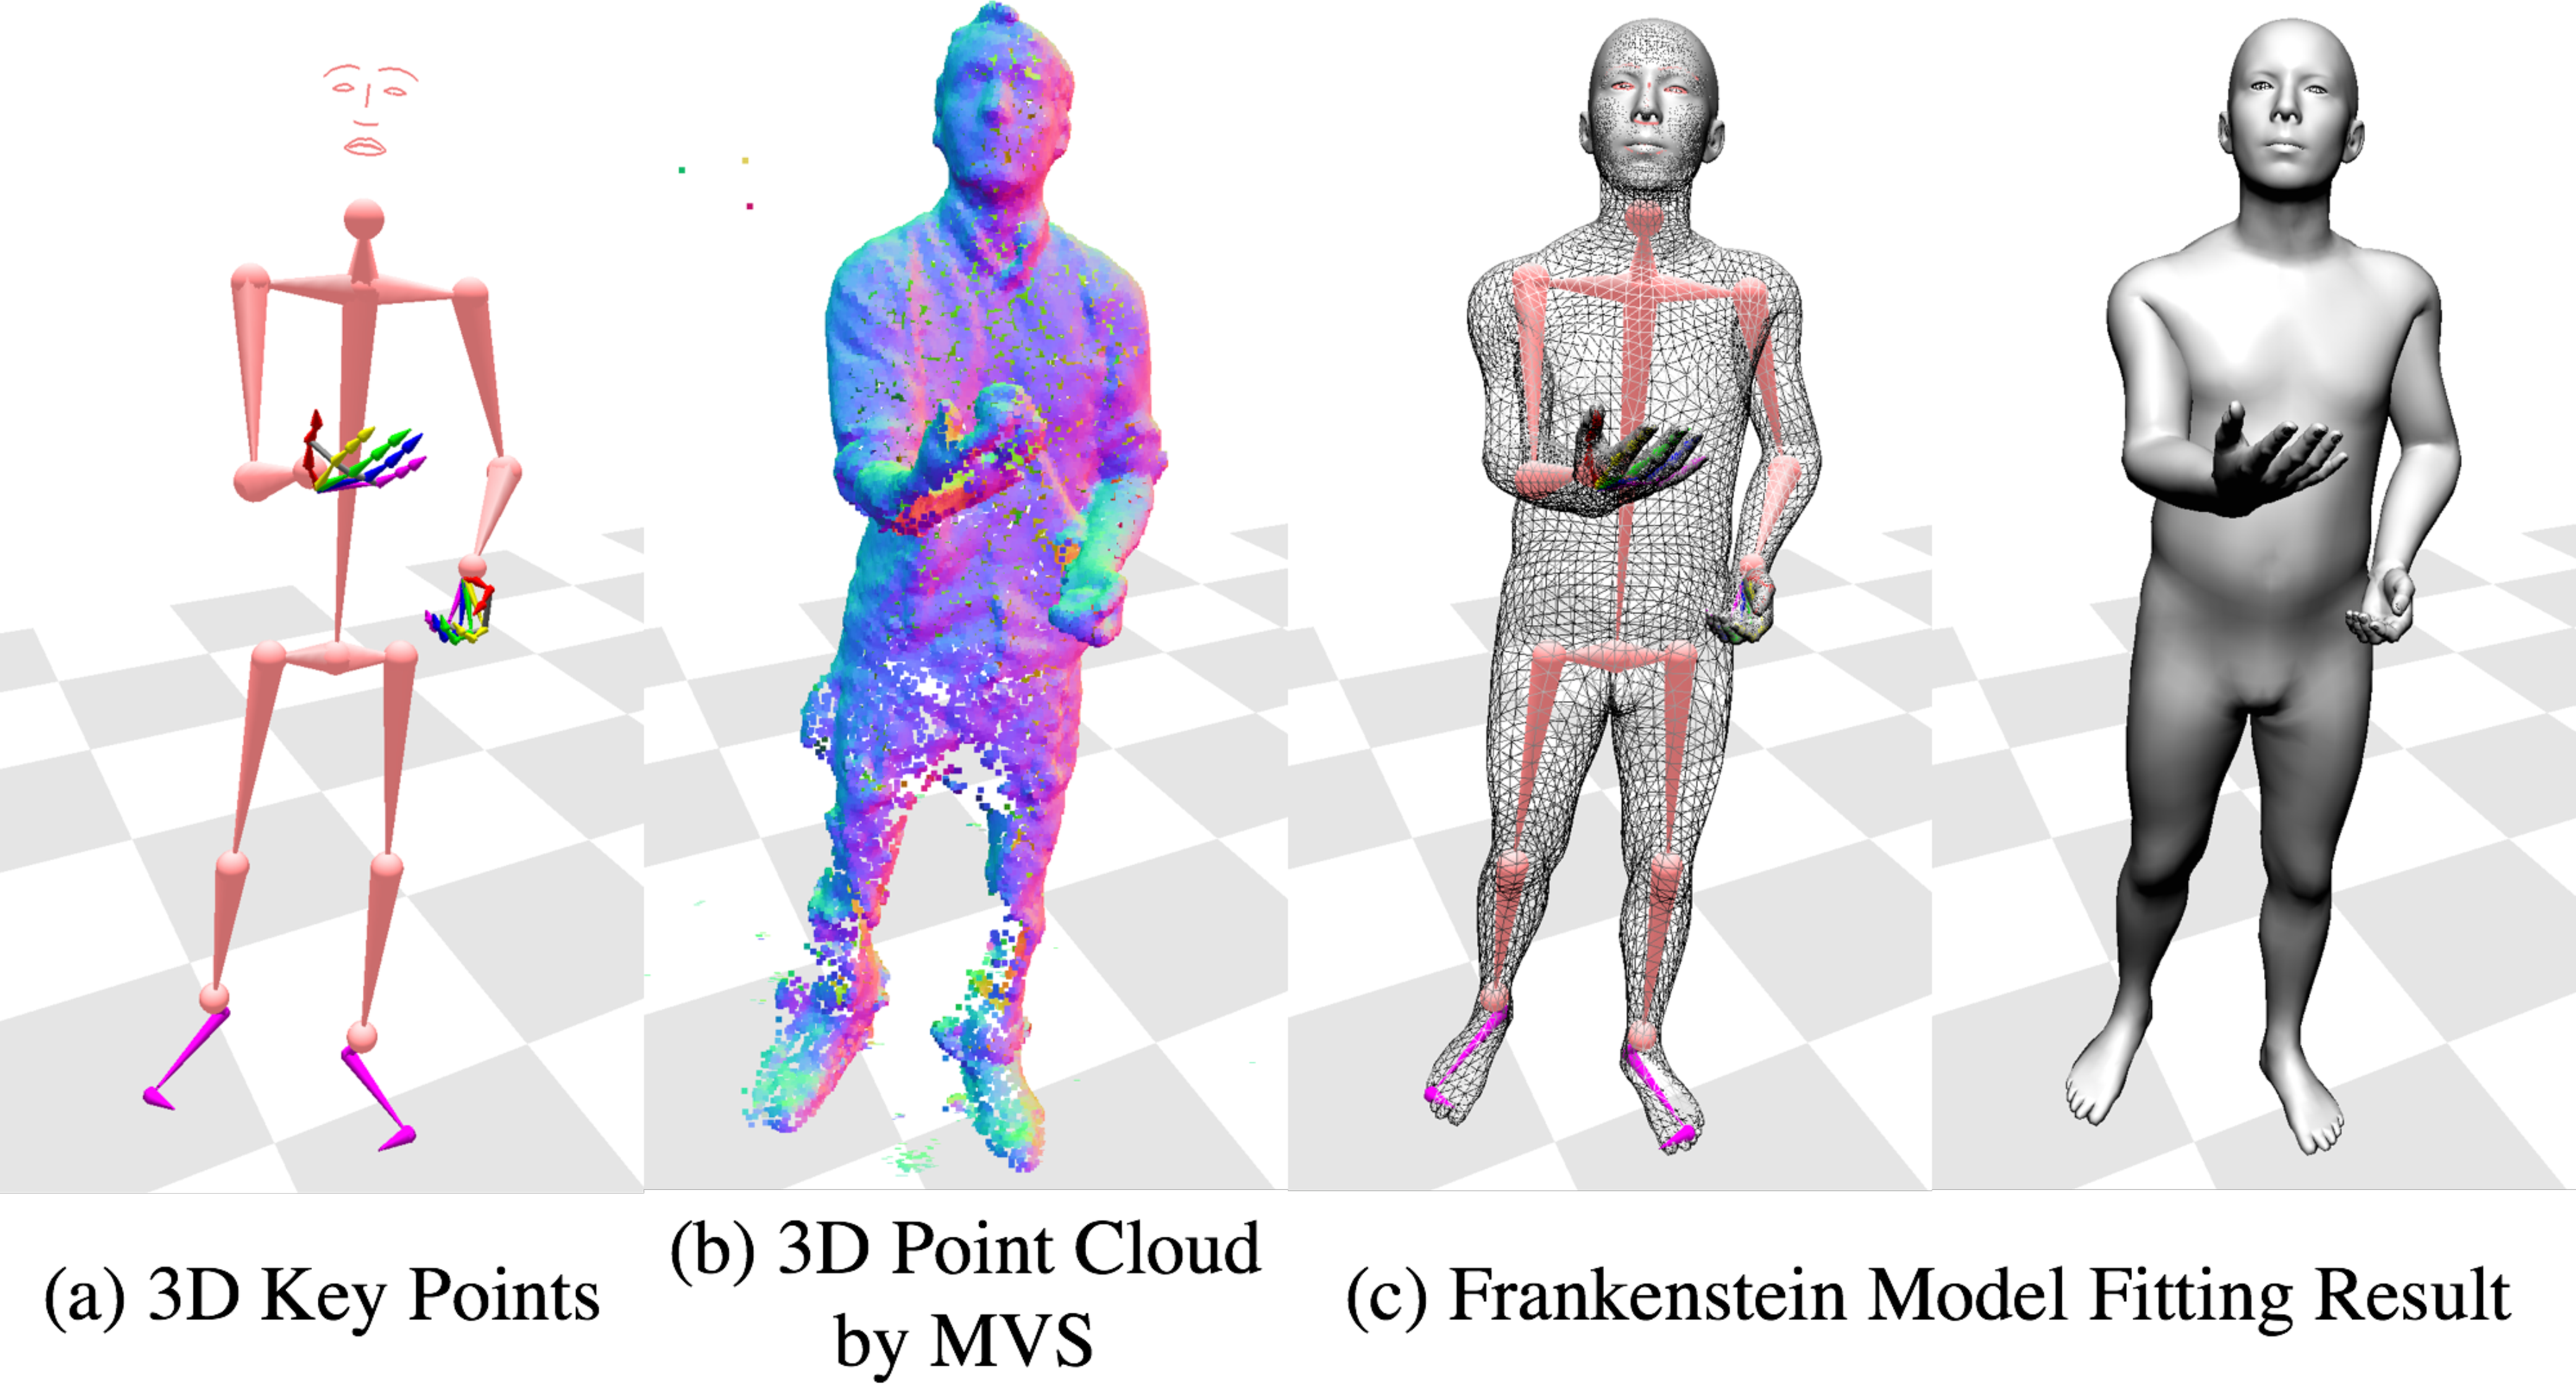
\includegraphics[width=\columnwidth]{tbc_figures/3Dmeasurements_legend2}
	\caption{Fitting Frank: The optimization takes, as input, (a) 3D keypoints, and (b) point clouds, and produces (c) a fitted skeleton and mesh as output.}
	\label{fig:3dlandmarks_model_fitting}
\end{figure}

%\begin{figure}[t]
%	\includegraphics[width=\columnwidth]{fig/modelAlignment}		\includegraphics[width=\columnwidth]{fig/modelAlignment2}
%	
%	\caption{Template model alignment to pre-compute correspondences}
%	\label{fig:modelAlignment}
%\end{figure}
%

%
%\subsection{Full Body Model}
%To recap, the full body model is parameterized by the following variables, which define the final position of each of the model's vertices in world coordinates:
%\begin{center}
%	\begin{tabular}{|c|c|c|} \hline 
%		Symbol & Meaning & Size \\ \hline\hline
%		$\mathbf{a}$ & Body shape coefficients & $10$\\ \hline
%		$\boldsymbol{\theta}$ & Body pose & $3\times 24$\\ \hline
%		$\mathbf{c}$ & Face shape coefficients & $150$ \\ \hline
%		$\mathbf{e}$ & Facial expression coefficients & $200$ \\ \hline
%		$\boldsymbol{\phi}^r$ & Right hand pose & $3\times 16$ \\ \hline
%		$\boldsymbol{\phi}^l$ & Left hand pose & $3\times 16$ \\ \hline
%		$\boldsymbol{s}$ & Hand scale parameters & $3\times 16$ \\ \hline
%		$\boldsymbol{t}$ & Global translation & $3$ \\ \hline
%		\hline
%	\end{tabular}
%\end{center}
%While the number of facial coefficients is larger than the degrees of freedom of other parts of the body, it should be noted that these parameters are heavily constrained by a prior, and, in fact, almost all of the variation in the training set is captured within approximately the first 60 coefficients. 
%
%Conceptually, the parameter set can be split into two categories. One set of parameters are static shape or {\em identity} parameters, including body shape, face shape, and hand scaling factors, which do not vary with time (e.g., bone lengths): 
%\begin{align}
%\mathcal{S} = \{\mathbf{a}, \mathbf{c}, \mathbf{s} \}.
%\end{align}
%The remaining parameters are per-frame {\em expression} parameters, including body pose, hand pose, facial expression, and global orientation and translation, 
%\begin{align}
%\mathcal{E}_t = \{ \boldsymbol{\theta}_t, \mathbf{e}_t, \boldsymbol{\phi}^r_t, \boldsymbol{\phi}^l_t,  \mathbf{t}_t \}.
%\end{align}
%This set of parameters is inherently dynamic and we index it with the sub-index $t$ to indicate that they are time-varying. To simplify the exposition, we will abstract away the details of each of the models used and instead denote the concatenated set of vertices,
%\begin{align}
%\mathbf{V}_t = [ \mathbf{V}_b, \mathbf{V}_f, \mathbf{V}_{hr}, \mathbf{V}_{hl} ] = B( \mathcal{S}, \mathcal{E}_t ),
%\end{align}
%where $\mathbf{V}_t\in\mathds{R}^{3\times V}$ with $V$ the total number of vertices, and the function $B(\cdot)$ maps from the combined model parameters, including static and per-frame parameters, to the full configuration of vertices for the body, face, and hands.

\subsection{Objective Function}

We initially fit every frame in the sequence independently. For clarity, we drop the time index from the notation and describe the process for a single frame, which optimizes the following cost function:
\begin{align}
\label{eq:fitting_franken}
E\big( \boldsymbol{\theta}^U, \boldsymbol{\phi}^U, \boldsymbol{t}^U \big) = E_\textrm{keypoints} + E_\textrm{icp} + E_\textrm{seam} +E_\textrm{prior}
\end{align}
We use Levenberg-Marquardt with the Ceres Solver library~\cite{ceres-solver} with multiple stages to avoid local minima. See the supplementary material for the details.

\textbf{Anatomical Keypoint Cost:} The term $E_\textrm{keypoints}$ matches 3D keypoint detections, which are in direct corresponce to our mesh models. This term includes joints (or end effectors) in the body and hands, and also contains points corresponding to the surface of the mesh (e.g., facial keypoints and the tips of fingers and toes). Both of these types of correspondence are expressed as combinations of vertices via a regression matrix $\mathbf{J}\,{\in}\,\mathds{R}^{C\times N^U}$, where $C$ denotes the number of correspondences and $N^U$ is the number of vertices in the model. Let $\mathcal{D}$ denote the set of available detections in a particular frame. The cost is then:
%We denote the aggregation of all 3D keypoints at time $t$ as $\mathbf{Y}_t$ and denote the aggregation of all corresponding joints and surface vertices as $\mathbf{V}_t$
\begin{align}
E_\textrm{keypoints} = \lambda_\textrm{keypoints} \sum_{i\in\mathcal{D}}|| \mathbf{J}_i \mathbf{V} - \mathbf{y}_i^T ||^2,
\label{eq:detection_eq}
\end{align}
where $\mathbf{J}_i$ indexes a row in the correspondence regression matrix and represents an interpolated position using a small number of vertices, and $\mathbf{y}_i\,{\in}\,\mathds{R}^{3 \times 1}$ is the 3D detection. The $\lambda_\textrm{keypoints}$ is a relative weight for this term.

\textbf{ICP Cost:} The 3D point cloud measurements are not a priori in correspondence with the model meshes. We therefore establish their correspondence to the mesh using Iterative Closest Point (ICP) during each solver iteration. 
We find the closest 3D point in the point cloud to each of the mesh vertices, and compute the point-to-plane residual, i.e., the distance along the normal direction,
\begin{align}
E_\textrm{icp} = \lambda_\textrm{icp} \sum_{\mathbf{v}_j \in \mathbf{V}^U} \mathbf{n}(\mathbf{x}_{j^*})^T (\mathbf{x}_{j^*} - \mathbf{v}_j ),
\end{align}
where $\mathbf{x}_{i^*}$ is the closest 3D point to $j$-th vertex $\mathbf{v}_j$,  $\mathbf{n}(\cdot)\in\mathds{R}^3$ represents the point's normal, and $\lambda_\textrm{icp}$ is a relative weight for this term. 
%Some details

%
%\begin{align}
%i^*= \operatorname{arg} \operatorname{min}_i  || \mathbf{x}_i - \mathbf{v}_j ||^2,
%\end{align}
%where $\mathbf{x}_{i^*}$ is the closest 3D point to vertex $j$, where $\mathbf{v}_j$ is a vertex\footnote{We do not consider some parts (around hands and face), as depth sensor resolution is too low to improve the estimate. These parts are excluded by a mask.} in $\mathbf{V}^U$ of the Frank model. To ensure that this is a correct correspondence, we use thresholds for the distance and normals during the correspondence search.
%
%Finally, for each vertex~$j$ we compute the point-to-plane residual, i.e., the distance along the normal direction,
%\begin{align}
%E_\textrm{icp} = \lambda_\textrm{icp} \sum_{\mathbf{v}_j \in \mathbf{V}^U_t} \mathbf{n}(\mathbf{x}_{i^*})^T (\mathbf{x}_{i^*} - \mathbf{v}_j ),
%\end{align}
%where $\mathbf{n}(\cdot)\in\mathds{R}^3$ represents the point's normal, and $\lambda_\textrm{icp}$ is a relative weight for this term. 

\textbf{Seam Constraints:} The part models composing the Frank model are rigidly linked by the skeletal hierarchy. However, the independent surface parameterizations of each of the part models may introduce discontinuities at the boundary between parts (e.g., a fat arm with a thin wrist). To avoid this artifact, we encourage the vertices around the seam parts to be close by penalizing differences between the last two rings of vertices around the seam of each part, and the corresponding closest point in the body model in the rest pose expressed as barycentric coordinates. %See the supplementary materials for details.
% with $\mathbf{B}_i\,{\in}\,\mathds{R}^{1\times N^B}$ (where $\mathbf{B}_i\mathbf{1}_{N^B}{=}1$), and similarly for the right hand and face.
%\begin{align}
%E_\textrm{seam} = &|| \mathbf{V}_{lh:B} - \mathbf{Y}_{B:lh} ||^2 +\\
% &|| \mathbf{V}_{rh:B} - \mathbf{Y}_{B:rh} ||^2 +\\
%  &|| \mathbf{V}_{F:B} - \mathbf{Y}_{B:F} ||^2,
%\label{eq:glue_constraints}
%\end{align}
%
% \begin{align}
% E_\textrm{seam} = &\sum_{(i,j)\in\mathcal{C}^{LH}} || \mathbf{B}_i\mathbf{V}^B - (\mathbf{v}^{LH}_{j})^T ||^2 +\\
%  &\sum_{(i,j)\in\mathcal{C}^{RH}} || \mathbf{B}_i \mathbf{V}^B - (\mathbf{v}^{RH}_{j})^T ||^2 +\\
%   &\sum_{(i,j)\in\mathcal{C}^{B}} || \mathbf{B}_i \mathbf{V}^B - (\mathbf{v}^{F}_{j})^T ||^2,
% \label{eq:glue_constraints}
% \end{align}
%\begin{align}
%E_\textrm{glue} = &\sum_{(i,j)\in\mathcal{C}^{LH}} || \mathbf{v}^B_{i} - \mathbf{v}^{LH}_{j} ||^2 +\\
% &\sum_{(i,j)\in\mathcal{C}^{RH}} || \mathbf{v}^B_{i} - \mathbf{v}^{RH}_{j} ||^2 +\\
%  &\sum_{(i,j)\in\mathcal{C}^{B}} || \mathbf{v}^B_{i} - \mathbf{v}^{F}_{j} ||^2,
%\label{eq:glue_constraints}
%\end{align}
% where the set $\mathcal{C}^{LH}$ contains correspondences $(i,j)$ where $j$ indexes the last two rings of vertices around the seam of the left hand, and $i$ denotes the corresponding closest point in the body model in the rest pose expressed as barycentric coordinates with $\mathbf{B}_i\,{\in}\,\mathds{R}^{1\times N^B}$ (where $\mathbf{B}_i\mathbf{1}_{N^B}{=}1$), and similarly for the right hand and face.

\textbf{Prior Cost:} 
Depending on the number of measurements available in a particular frame, the set of parameters of $M^U$ may not be determined uniquely (e.g., the width of the fingers). More importantly, the 3D point clouds are noisy and cannot be well explained by the model due to hair and clothing, which are not captured by the SMPL and FaceWarehouse meshes, resulting in erroneous correspondences during ICP. Additionally, the joint locations of the models are not necessarily consistent with the annotation criteria used to train the 2D detectors. We are therefore forced to set priors over model parameters to avoid the model from overfitting to these sources of noise, $E_\textrm{prior} = E^F_\textrm{prior} + E^B_\textrm{prior} + E^H_\textrm{prior}$.
% \begin{align}
% E_\textrm{prior} = E^F_\textrm{prior} + E^B_\textrm{prior} + E^H_\textrm{prior}
% \end{align}
The prior for each part is defined by corresponding shape and pose priors, for which we use zero-mean standard normal priors for each parameter except for scaling factors, which are encouraged to be close to 1. %Details and relative weights can be found in supplementary materials.
% All PCA derived parameters are penalized with the corresponding variance, which by construction 

% of our basis is:
% \begin{align}
% E_\textrm{prior}^F &= \lambda_{SF} ||\phi^F||^2 + \lambda_{PF} ||\theta^F||^2\\
% E_\textrm{prior}^B &= \lambda_{SB} ||\phi^B||^2 + \lambda_{PB} ||\theta^B||^2\\
% E_\textrm{prior}^H &= \lambda_{SH} ||\phi^H-1||^2 + \lambda_{PH} ||\theta^H||^2
% \end{align}
% where, for simplicity, we penalize pose parameters that deviate from the rest pose with a small weight, and we encourage hand scaling factors to be close to 1.
%\begin{align}
%E_\textrm{prior}^F = E^F_\textrm{prior}(\phi^F) + E^F_\textrm{prior}(\theta^F)\\
%E^F_\textrm{prior}(\phi^F) = {\phi^F}^T\phi^F\\
%E^F_\textrm{prior}(\theta^F) = {\theta^F}^T\theta^F,
%\end{align}
% and similarly for other part model parameters. We use different weights for the priors on different parts ($\lambda_{SF}=\lambda_{SH}=10^{-2}$, $\lambda_{SB}=10^{-2}, \lambda_{PF}=10^{-4}, \lambda_{PB}=10^{-6}$, and $\lambda_{PH}=10^{-7}$).

%face_shape 1e-4
%body shape 1e-2
%hand shape 1e-4


%face_exp =1e-4
%body pose 1e-6
%hand pose =1e-7


%\subsection{Optimization Procedure}
%The complete model is highly nonlinear. Therefore, instead of optimizing the complete model initially, we fit the model in phases, starting with a subset of measurements and strong priors that are relaxed as optimization progresses. Model fitting is performed on each frame independently, and we use Levenberg-Marquardt with the Ceres Solver library~\cite{ceres-solver}. See the supplementary material for the details.

%and due to the limited degrees of freedom of the skeletal joints, the optimization can get stuck in bad local minima. 
% Similarly, the ICP term requires a reasonable initial alignment between the model and measurements to find correspondences. 
%Therefore, instead of optimizing the complete model initially, we fit the model in phases, starting with a subset of measurements and strong priors that are relaxed as optimization progresses.

%Model fitting is performed on each frame independently. To initialize the overall translation and rotation, we use four keypoints on the torso (left and right shoulders and hips) without using the ICP term, and with strong weight on the priors. Once the torso parts are approximately aligned, we use all available keypoints of all body parts, with small weight for the priors. The results at this stage already provide reasonable motion capture but do not accurately capture the shape (i.e., silhouette) of the subject. Finally, the entire optimization is performed including the ICP term to find correspondences with the 3D point cloud. We run the final optimization two times, finding new correspondences each time. For the optimization we use Levenberg-Marquardt with the Ceres Solver library~\cite{ceres-solver}. 

%During the optimization, we ignore keypoints if they do not have confident triangulations (i.e., low detection scores or insufficient inlier views). We also do a visibility check to avoid corresponding mesh vertices with point cloud points that have been reconstructed from cameras unlikely to have seen that mesh vertex. For the optimization we use Levenberg-Marquardt with the ceres library. 

%After reconstructing total motion per frame, we also can reconstructing multiple frame together by using the same 54

%
%\subsection{Discussion}
%\label{Franken:discussion}
%We find that total motion capture with the Frankenstein model already produces compelling results, as shown in the accompanying video. However, there are several aspects which need improvements: 1) the model only produces shapes without hairs and clothing, very different from the natural interactions we aim to capture; 2) model optimization is complex, and requires additional optimization parameters to keep the parts connected without artifacts, making implementation complicated, and 3) the definition of joints for the 2D detectors is different from the actual location of the joints in the 3D skeleton, resulting in a nonzero cost function even for the correct pose.

%
%
%\subsection{Fitting Cost Function}	
%The parameters of the full body model $B(\cdot)$ are fit to match the available 3D measurements in the Panoptic Studio by minimization of a suitable cost function. These measurements can either be triangulated 3D detections that are in correspondence with the model (i.e., they have a semantic label attached, e.g., ``left elbow'') or simply represent a reconstructed 3D point (from either stereo or a depth sensor) with no additional information. These latter points could potentially correspond to an arbitrary location on the surface of the body, but it is also possible that they do not belong to the body at all (e.g., other people, objects). Therefore, the two types of measurements must be handled differently, and we refer to each of these as $E_{\textrm{detection}}$ and $E_{\textrm{icp}}$ respectively. Additionally, the cost function will include priors over both the shape parameters, and the expression parameters capturing the pose at any given time instant. A high-level description of the optimization problem is then to find the parameters that minimize the cost function:
%%\begin{align}
%%\{ \mathbf{\theta}^U, \mathbf{\phi}^U_{1..T}, \mathbf{t}^U_{1..T} \}^*= \underset{{\{ \mathbf{\theta}^U, \mathbf{\phi}^U_{1..T}, \mathbf{t}^U_{1..T}\}}} {\arg\min} E_\textrm{detection} + E_\textrm{icp} 
%%\label{eq:totalCost}
%%\end{align}
%%+ E_\textrm{shape prior} + E_\textrm{expression prior},
%where $T$ is the total number of frames. We describe each of these error terms in more detail in the following sections.
%
%\subsubsection{Anatomical Landmark Cost}
%For anatomical landmark points, we enforce the constraint that their measured 3D position should match that of the corresponding point on the mesh models. Our detectors fire both on internal points (the joints of the body and hands) as well as on points that are on the surface of the body (e.g, the facial landmarks). To treat all corresponded points in the same way, we define each of these positions on the mesh as a linear combination of a small set of vertices on the respective models. We formulate this as the action of a linear observation matrix $\mathbf{O}$,
%\begin{align}
%\boldsymbol{r} =  \mathbf{O} \operatorname{vec}(\mathbf{V}_t) - \operatorname{vec}(\mathbf{Y}_t)
%\end{align}
%with $\mathbf{Y}_t\in\mathds{R}^{3\times n_{\textrm{det}}}$ the set of triangulated 3D detections for frame $t$, $n_{\textrm{det}}$ the number of detections, and $\mathbf{O}\in\mathds{R}^{n_{\textrm{obs}}\times 3V}$ the observation matrix, where $n_\textrm{obs}=3n_\textrm{det}$. Here, $\boldsymbol{r}$ is the vector of residuals, i.e., the mismatch between the model and the observed point. Not all the correspondences are always available, nor should all residuals be weighted equally, so we write the final cost due to detections as
%\begin{align}
%E_\textrm{detection} = \frac{1}{2} \mathbf{r}^T \mathbf{W} \mathbf{r},
%\label{eq:detection_eq}
%\end{align}
%with $\mathbf{W}$ a weighting matrix. Nominally, $\mathbf{W}$ corresponds to the inverse covariance of the residuals; however, in practice, we approximate this as a diagonal with weight $c_i$ for the residual entries corresponding to detection $i$, where $c_i\in[0,1]$ is the detection confidence of that detection (and $0$ if the detection is missing). 
%
%
%
%
%
%
%The parameters of the full body model $B(\cdot)$ are fit to match the available 3D measurements in the Panoptic Studio by minimization of a suitable cost function. These measurements can either be triangulated 3D detections that are in correspondence with the model (i.e., they have a semantic label attached, e.g., ``left elbow'') or simply represent a reconstructed 3D point (from either stereo or a depth sensor) with no additional information. These latter points could potentially correspond to an arbitrary location on the surface of the body, but it is also possible that they do not belong to the body at all (e.g., other people, objects). Therefore, the two types of measurements must be handled differently, and we refer to each of these as $E_{\textrm{detection}}$ and $E_{\textrm{icp}}$ respectively. Additionally, the cost function will include priors over both the shape parameters, and the expression parameters capturing the pose at any given time instant. A high-level description of the optimization problem is then to find the parameters that minimize the cost function:
%\begin{align}
%{\{ \mathcal{S}, \mathcal{E}_1,\dots, \mathcal{E}_T\}} = \arg \min_{\{ \mathcal{S}, \mathcal{E}_1,\dots, \mathcal{E}_T\}}\ E_\textrm{detection} + E_\textrm{icp} + E_\textrm{shape prior} + E_\textrm{expression prior},
%\end{align}
%where $T$ is the total number of frames. We describe each of these error terms in more detail in the following sections.
%
%\subsection{Optimization Procedure}
%
%
%F()
%
%
%
%Our complete model is highly nonlinear, has a large number of unkown parameters, and inportantaly some of the measurement might be missing. There, instead optimizing complete model together at the beginning, we use an iterative scheme by fitting the model with several phase starting with a subset of measurement. This type of approach usually tend to suffer from a local minima if the initial phase of the optimization failed, but we found that our method don't have this issue because the ininitialization from the intial mesurement (anatomical landmark) provide a good initialization. To this end, we optimize complete model using the result of previous phase as an initial which works well especially to find correspondences in ICP. 
%
%\subsubsection{Scale Search}: We first compute scales from entire skeletons. For the body, scale is related to the identity model.
%
%\subsubsection{Per-Frame Optimization}: Per-Frame optimization provide robustness for any complicated motion since it doesn not suffer from error accumulation. The goal of this optimization is to provide a good initialization for the next step, and we fit the model only if ``enough" measurement is availble. 
%
%Given the landmarks for face, hand, and body, we fit each template model seperately for the joint. Here we need to consider the DoF of the model and the measuremnt constraint to avoid an explosion of the fitting. 
%
%For the face, we use 10?? parameters and so it has enough contraint if more than 3 points are available. So in general, face is fine
%
%For the hand, we only fit the hands only if all the hand joint measurment is valid. Since we constraig the angles for each hand (most of them has only 1 dof), we notice it is sufficient.  The Scale factor should be also computed (preprocessing??, any big difference?)
%
%
%SMPL body model has both shape and motion paramaeters, which cannot be constrained by joints. So we use a prior for the shape and the pose to handle this, while we constarint some degree of freeedom for knees and elbows. 
%
%When we are optimizing SMPL body, we also put addtional constraing between body and face and hand so that they are attached together. 
%This happen only if the hand and face are valid. 
%
%\section{Out-of-Model Space Deformation and }
%One of the good advantage of using skeletons and per-frame fitting is that they are completely independent from motion and topological changes which is challenging issues in the existing method. 
%
%After per-frame model fitting, we can additionally deforme the model to cover the surface out of the model space. To handle this in a simple way, we first compute the additional deformation parameters for each vertex along normal direction for each point. Ideally this deformation factor should be determined by finding the corresponding surface location. However, due to the noisy pont cloud status, ths would produce erroneous results, as shown in Fig. XX. 
%
%There are two reasons: 1) wrong correspodence is happens if body limbs are close to the body; 2) If there is no correspondence, the part is not deformed. 
%
%We solve this is by applying a conservative deformation, meaning that we do the deformaiton only the correspondence is reliable. The complete deformation can be complete by fusing the deformation factors across time. That is we update the deformation factor in the canoncial space only if the part is visible from sensors, and to do that we do a visibility search. 
%
%After generating the deformation, we simply rerun the model fitting with ICP, which produce better skeleton fit by handling out of space shape space. 
%
%
%\section{Tracking and Iteration}
%The perframe detection doesn't suffer from error accumulation, but it sometimes failed dut to the severe pose detection failures, and have missting hand, face, and bodies. We solve this issue by using temporal tracking. 
%
%
%Our temporal tracking is based on a short term tracking (3 frames) because long term tracking is often a very challenging problem. So we only track 3 frames (backward, forward from the current frame) and propagate information based on that. 
%
%A hole of a single frame can be directly filled by this propagation, and longer holes also can be filled by applying this multiple times. We do iteration until there is no more update in the propagation. 
%
%We also do this for stabing skeletons temoprally, by averaging the propagated information with the original information if there is, similar to the method of Joo 17
%
%The tracking is done for the all the projected vertices of the meshes. We do visibility check and only aggregate optical flow information, and optimize the vertice position based on that. Our optimization is done for the pose parameter only by fixing shape parameters. 

%
%How to find correspondence between each template vertex and a target location?
%
%Instead of nearest neighbor,  we use normal directional location by averaging a set of nearest neighbor (selected by a sphere and normal filtering).
%
%\begin{figure}[h]
%	\includegraphics[width=\columnwidth]{fig/corres1}
%		\caption{Deformation Challenge}
%	\label{fig:corres_failure}
%\end{figure}
%
%However, as shown in Fig.~\ref{fig:corres_failure}, this cannot handle the case where limbs and body are very close each other. This also affects the performance of ICP and subsequence parameter optimization.
%
%\subsection{Fusing Deformation across frame}
%
%
%
%\section{Fusion with Tracking}


% !TEX encoding = UTF-8 Unicode
% !TEX root = ../thesis.tex


\begin{figure}[t]    
\centering
	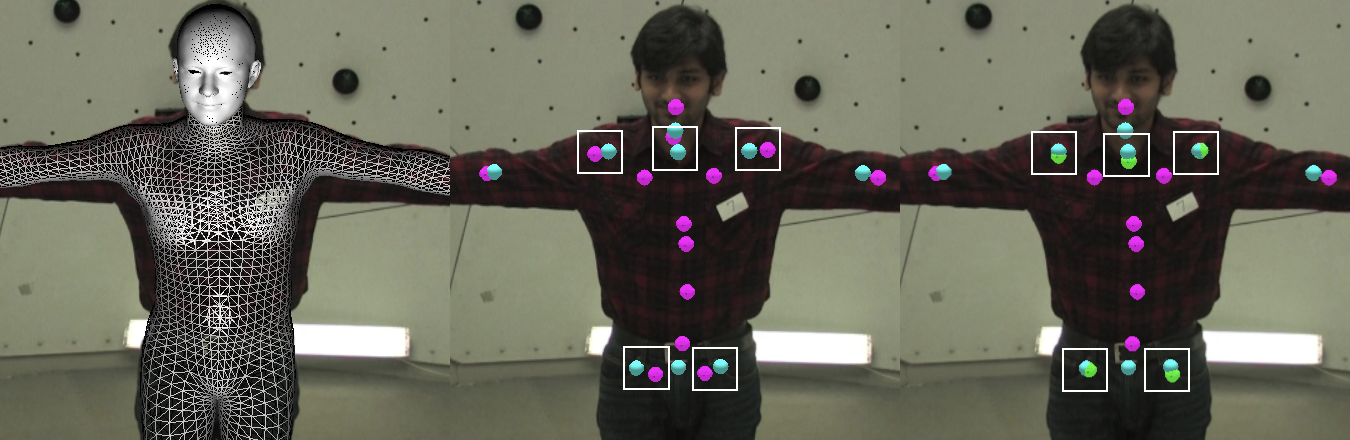
\includegraphics[width=\columnwidth]{tbc_figures/Jointregression_detectionTarget_nospace}    
	%\includegraphics[width=0.9\columnwidth]{fig/detectionTarget_legend}   
	\caption{Regressing detection target 3D positions. (Left) The template model is aligned with target object; (Mid.) The torso joints of the template model (magenta) have discrepancy from the joint definitions of 3D keypoint detection (cyan); (Right) The newly regressed target locations (green) are more consistent with 3D keypoint detections.}
	\label{fig:jointRegression}
\end{figure}
%
%
%\begin{figure}[t]    
%	\includegraphics[width=\columnwidth]{fig/Jointregression_coloradjus}  
%	\label{fig:adam_jointRegression}
%	\caption{We train a new regression function to compute joints from mesh vertices based on the reconstructed hundreds people's examples. (a) Projected mesh on an example image showing that the template model is aligned with target object. (b) The torso joints of the template model (magenta) have discrepancy from the joint definition of 3D detection measurements (cyan). (c) Newly regressed joints of our method are shown as green (d) Our joints definition (green)is more consistent to the joints from detection (cyan). }
%\end{figure}	

%\section{Building Total Model}
\section{Creating Adam}
We derive a new model, Adam, enabling total body motion capture with a simpler parameterization than the part-based Frank model. In particular, this new model has a single joint hierarchy and a common parameterization for all shape degrees of freedom, tying together the face, hand, and body shapes and avoiding the need for separate part parameterizations or seam constraints. To build the model, it is necessary to align the reconstructed meshes with all body parts (face, body, and hands) of diverse subjects where the model can learn the variations. To do this, we leverage our Frank model and apply it on a dataset of 70 subjects where each of them performs a short range of motion in a multiview camera system. We select 5 frames for each person in different poses, resulting in 350 meshes, and reconstruct them with our Frank model, producing aligned meshes with joint locations to build Adam. Because we derive the model from clothed people, the blendshapes explain variations of clothing at a coarse level.% due to the bulk of clothes and hair.

%while wearing everyday clothing. During the capture, we asked them to perform a T-pose and an action of their choosing. We selected 5 frames for each person with different poses and fit the Frankenstein model to each frame independently, which are then used to build Adam. Because we derive the model from clothed people, the linear shape blendshapes explain some variation in geometry due to the bulk of clothes and hair, which leads to better surface matching during ICP.
%We build a new model, named the TOTAL MODEL, to capture to solve the issued arising in the Frankenstein model. To achieve this, we collect a large scale humna dataset with natural hairs, clothing, and motions. We use the Frankenstein Model to compute the motion and shape for the people, and also reconstruct the out-of-model shapes by computing normal-direction delta shape parameters. To this end, we build a new linear blend shapes to cover the clothing and hairs. We also additional tuned the joint location to be consistent with detection cost. The final optimization framework is much simpler and more generally usable than the Frankenstein models. 
%We collect a short range of motion sequence from 70 people,  Examples are shown in Fig.~\ref{fig:compare_franken_adam}.


%\subsection{Reconstructing out-of-model space}
\subsection{Fitting Clothes and Hair}
%The output of the previous fitting still contains shapes in the model space. 
The Frank model captures the shape variability of human bodies and faces, but does not account for clothing or hair, since it keeps the original model space of part models (\cite{Loper2015} and \cite{cao2014facewarehouse}). To learn a new set of linear blendshapes that better capture the rough geometry of clothed people and also roughly model hair, we need the meshes to match the geometry of the source data more accurately. For this purpose, we deform the meshes outside of the shape-space along each the normal direction of each vertex. For each vertex $\mathbf{v}_i $ in the Frank model, the deformed mesh vertex $\tilde{\mathbf{v}}_i$ is represented as:
\begin{align}
\tilde{\mathbf{v}}_i  =  \mathbf{v}_i  + \mathbf{n}(\mathbf{v}_i) \delta_i,
\end{align}
where $\delta_i \in \mathds{R} $ is a scalar displacement meant to compensate for the discrepancy between the Frank model vertices and the 3D point cloud, along the normal direction at each vertex. 
% However, directly computing this from closest-point correspondences can produce severe artifacts, as the 3D point clouds are noisy and contain large holes due to failed stereo matching. We therefore use a Laplacian shape prior\cite{} to regularize the deformations and introduce visibility and normal matching constraints to reject incorrect correspondences. 
%Finally, we run the optimization over multiple frames together with a shared $\Delta$ parameters
%\textbf{Laplacian Shape constraints}
We pose the problem as a linear system,
% transform the current vertex $\mathbb{V}$ to be close to the target point cloud set $\mathbf{P}$, with Laplacian of the mesh is maintained:
%\begin{align}
%\mathbf{V} +N\cdot\Delta = \mathbf{P}\\
%L\cdot \left( \mathbf{V} + N\cdot\Delta \right) - L\cdot\mathbf{V} = 0
%%L\cdot \left( N\cdot\Delta \right) = 0
%\end{align}
%Since all terms are linear, we can concatenate them to build a linear system:
%
\begin{align}
\label{eq:delta_recon}
\begin{pmatrix} \mathbf{N}^T  \\ (\mathbf{W} \mathbf{L} \mathbf{N})^T  \end{pmatrix} \Delta
= \begin{pmatrix} (\mathbf{P} - \mathbf{V}^U)^T \\ \mathbf{0} \end{pmatrix},
\end{align}
where $\Delta\in\mathds{R}^{N^U}$ contains the stacked per-vertex displacements, $\mathbf{V}^U$ are the vertices in the Frank model, $\mathbf{P}\in\mathds{R}^{N^U\times 3}$ are corresponding point cloud points, $\mathbf{N}\in\mathds{R}^{N^U\times 3}$ contains the mesh vertex normals, and $\mathbf{L}\in\mathds{R}^{N^U\times N^U}$ is the Laplace-Beltrami operator to regularize the deformation. We also use a diagonal weight matrix $\mathbf{W}\in\mathds{R}^{N^U\times N^U}$ to avoid large deformations where the 3D point cloud has lower resolution than the original mesh, such as details in the face and hands. %After reconstructing $\Delta$, the generated output models shows better 
% \textbf{Visibility Maps: } 
% Deforming out of model space can introduce artifacts if false correspondences are established with the noisy point clouds that we get from our limited resolution cameras. 
% % This is particularly true with the point cloud reconstructions we were able to get with the limited resolution of our multicamera system. 
% Problematic regions include joint regions, where association can match points to a different body part. To avoid this, we discard ``unreliable'' correspondences using a visibility heuristic. We compute the visibility of every vertex from the cameras used to reconstruct the point cloud, and use this as a reliability measure: if a vertex is not visible from sufficient cameras, it is unlikely to have a corresponding 3D match, so we do not correspond such difficult areas (e.g., below the arms, between the legs). 

% \textbf{Multi Frame Fitting: } To further reduce noise, we solve for the surface $\Delta$ using multiple frames simultaneously. This can be done by stacking the linear constraints in Eq.~\ref{eq:delta_recon} obtained from multiple frames in a single system. 
%\begin{align}
%\begin{pmatrix} \mathbf{N}_1  \\ \mathbf{L}\cdot \mathbf{N}_2 \\ \mathbf{N}_2  \\ \mathbf{L}\cdot \mathbf{N}_1 \\ \cdots \end{pmatrix} \Delta
%= \begin{pmatrix} \mathbf{P}_1 - \mathbf{V}_1 \\ \mathbf{0}  \\ \mathbf{P}_2 - \mathbf{V}_2 \\ \mathbf{0} \\ \cdots \end{pmatrix}
%\end{align}

%\begin{figure}[t]	
%	\includegraphics[width=0.32\columnwidth,trim=800 80 500 90, clip]{fig/visibility_corres/visibility_5frames_1iter}
%	\includegraphics[width=0.32\columnwidth,trim=800 80 500 90, clip]{fig/visibility_corres/1_1iter_noVis}	
%	\includegraphics[width=0.32\columnwidth,trim=800 80 500 90, clip]{fig/visibility_corres/1_1iter_visibility_1frames}
%	%\includegraphics[width=0.24\columnwidth,trim=0 0 0 0, clip]{fig/visibility_corres/visibilityMap}	
%	
%	\caption{Delta Reconstruction Results. (a) Original Frankenstein model output; (b) Delta deformation without visibility map; (c) Delta deformation with visibility map; (D) color coded visibility map (blue with low visibility, and red with high visibility).}
%	\label{fig:deltarecon}
%\end{figure}
%

% \begin{figure}[t]    
% 	\includegraphics[width=\columnwidth]{fig/compare_franken_adam}    
% 	%\includegraphics[width=\columnwidth]{fig/compare_franken_adam2}    
% 	\caption{Comparison between the shape space of Frankenstein model and Adam model. For each example, (left) an input image; (middle) Frankenstein model fitting result; (right) Adam model fitting result with the same 3D measurements.}
% 	\label{fig:compare_franken_adam}
% \end{figure}

% Emphasize this section in the contribution. 
% There's a disconnect between the joints and the output of the detectors. Detector target regressor?

%\subsection{Regressing New Joint Locations}
\subsection{Detection Target Regression}
There exists an important discrepancy between the joint locations of the LBS model (i.e., the 3D centers of rotation for bone deformation) and the location of the keypoint detections (which come from manually annotated guesses of where the anatomical joints are in 2D images). This is shown in Fig.~\ref{fig:jointRegression}. This difference has the effect of pulling the model towards a bad fit even while achieving a low keypoint cost, $E_{\textrm{keypoints}}$, especially for shoulders and hips. We alleviate this problem by computing a new regression function, $\mathbf{\hat{J}}^A \in \mathds{R}^{J^A\times N^U}$, which relates the vertices in the body model to the expected location of 3D keypoint detections. However, to be able to learn these regressors, we require instances of the fitted model vertices as well as the 3D keypoint detections.


Therefore, we first fit the Frank model (with additional shape variations) using the original joint locations as detection targets, and obtain aligned meshes across all subjects. Based on these outputs, we can build the regression matrix using the  locations of 3D keypoint measurements as targets instead of Frank model's joint locations. Similar to the joint regression in SMPL~\cite{Loper2015}, we first select a subset of vertices in the proximity of each detection target, and estimate a fixed, sparse linear combination of these vertices that approximates the location of the 3D keypoint across all fitted meshes. This optimization is posed as an L1-regularized least-squares problem with non-negative constraints, where we additionally impose that the vertex weights sum to one, resulting in an interpolation. 

The results are shown in Fig.~\ref{fig:jointRegression}. Note that this new regressor is used only for the optimization in Eq.~\eqref{eq:detection_eq}, whereas the original joint regressor from SMPL~\cite{Loper2015}, $\mathbf{J}^A$, is used for LBS. However, we also add rows to the joint regression matrix to account for the additional finger joints, which we solve for in the same way. The resulting matrix is $\mathbf{J}^A \in \mathds{R}^{J^A\times N^U}$ where $N^U$ is the number of vertices of Adam (the same as Frank) and $J^A=61$ is the number of joints in Adam model including 21 body joints and 20 finger joints (including 5 finger tips) for each hand. 

 %a 3D detection, and then estimate a fixed, sparse linear combination of these vertices that approximates the location of the 3D keypoint across all fitted meshes. This is posed as as L1-regularized least squares problem with non-negative constraints, where we additionally impose that the vertex weights sum to one, resulting in an interpolation. We found that we achieved best results by solving this problem iteratively, starting from a large set of candidate vertices and then removing vertices with zero or low weights, and then repeating the procedure with the new candidate set until each detection uses fewer than 10 vertices as interpolators. These new regression weights are then used to generate correspondences to the detection targets in $E_\textrm{keypoints}$. 


%The problem can be alleviated by also fitting the mesh surface to the MVS point clouds using ICP. This leads to a better overall fit, but a higher $E_{\textrm{keypoints}}$ cost, as the SMPL joints and the 3D detections will no longer be perfectly aligned. 



%the relative location of the 3D detections with respect to the fitted mesh vertices by leveraging the the reconstructed 70 people data. This allows us to define new targets for the keypoint detection cost that, on average, are a better match for the location of the 3D detections with respect to the mesh model, as shown in Fig.~\ref{fig:jointRegression}. In particular, given the fitting results of 70 identities, we approximate the target 3D keypoint locations as a function of the final fitted mesh vertices following the procedure of~\cite{Loper2015} to find a sparse, linear combination of vertices that approximates the position of the target 3D keypoint. Note that we do not change the joint location used in the skeleton hierarchy during LBS deformation, only the regression matrices $\mathbf{J}_i$ in Eq.~\eqref{eq:detection_eq}. %This can be also applied on Farnkenstein model. 
%Original
%There exists a discrepancy between the SMPL body joint locations and the location of the keypoint detections used in the OpenPose body detector (i.e., a model joint vs. a detection joint). This affects mainly the shoulder and hip joints, which are not only difficult to annotate on clothed people, but are also difficult to model accurately in an LBS framework, which results in non-anatomical placements for these joints. This difference in their definition has the effect of pulling the Frankenstein model towards a bad fit even while achieving a low keypoint cost, $E_{\textrm{keypoints}}$. The problem can be alleviated by also fitting the mesh surface to the MVS point clouds using ICP. This leads to a better overall fit, but a higher $E_{\textrm{keypoints}}$ cost, as the SMPL joints and the 3D detections will no longer be perfectly aligned. We alleviate this problem by computing the relative location of the 3D detections with respect to the fitted mesh vertices by leveraging the the reconstructed 70 people data. This allows us to define new targets for the keypoint detection cost that, on average, are a better match for the location of the 3D detections with respect to the mesh model, as shown in Fig.~\ref{fig:jointRegression}. In particular, given the fitting results of 70 identities, we approximate the target 3D keypoint locations as a function of the final fitted mesh vertices following the procedure of~\cite{Loper2015} to find a sparse, linear combination of vertices that approximates the position of the target 3D keypoint.
% We follow a similar procedure as used in \cite{Loper2015} to define the location of SMPL joints as a function of mesh vertices. 
% We first select a subset of vertices in the proximity of a 3D detection, and then estimate a fixed, sparse linear combination of these vertices that approximates the location of the 3D keypoint across all fitted meshes. This is posed as as L1-regularized least squares problem with non-negative constraints, where we additionally impose that the vertex weights sum to one, resulting in an interpolation. We found that we achieved best results by solving this problem iteratively, starting from a large set of candidate vertices and then removing vertices with zero or low weights, and then repeating the procedure with the new candidate set until each detection uses fewer than 10 vertices as interpolators. These new regression weights are then used to generate correspondences to the detection targets in $E_\textrm{keypoints}$. 
%Note that we do not change the joint location used in the skeleton hierarchy during LBS deformation, only the regression matrices $\mathbf{J}_i$ in Eq.~\eqref{eq:detection_eq}. 

\subsection{Building the Shape Deformation Space}

After model fitting with $\Delta$ displacement, we warp each frame's surface to the rest pose, applying the inverse of the LBS transform. With the fitted surfaces warped to this canonical pose, we do PCA analysis to build a joint linear shape space that captures shape variations across the entire body. As in Section~\ref{subsection:face}, we separate the expression basis for the face and retain the expression basis from the FaceWarehouse model, as our MVS point clouds are of too low resolution to fit facial expressions.
%To do that, we first export all the meshed in the rest poses, where all the pose parameters are zeros. Then, we run the similar method as we used to build the linear space for face, in subsection \ref{subsection:face}.

%The mean pose and example linear subspaces are shown in Fig.\ref{fig:totallinearspace}. 
%The a model now can have shape variation for all parts, including body, hand, and face. The model also includes deformation of hair and clothing. That is this model can substitute parameters of $\phi^F$, $\phi^B$, and $\phi^H$. 
The Adam model is parameterized as:
\begin{align}
M^A (\boldsymbol{\theta}^A, \boldsymbol{\phi}^A, \boldsymbol{t}^A ) = \mathbf{V}^A
\end{align}
with $\mathbf{V}^A = \{ \mathbf{v}^A_i\}_{i=1}^{N^A}$ and $N^A{=}18540$ which is equal to the vertices in Frank, $N^U$. As in SMPL, the vertices of this template mesh are first displaced by a set of blendshapes in the rest pose, $\hat{\mathbf{v}}^A_i = \mathbf{v}^{A0}_i + \sum_{k=1}^{K_A} \mathbf{s}^k_{i} \phi^A_k,$ 
where $\mathbf{s}^k_{i}\in\mathds{R}^3$ is the $i$-th vertex of the $k$-th blendshape, $\phi^A_k$ is the $k$-th shape coefficients of $\boldsymbol{\phi}^A\in\mathds{R}^{K_b}$, and $K_A=40$ is the number of identity coefficients, $\mathbf{v}^{A0}$ is the mean shape and $\mathbf{v}^{A0}_i$ is its $i$-th vertex. Note that these blendshapes now capture variation across the face, hands, and body. These are then posed using LBS as in Eq.~\eqref{eq:full_lbs_pose} after obtaining joint locations by the joint regressor matrix $\mathbf{J}^A$. %We define the joints and weights for LBS followoing the part models, which is further explained in the supplementary material. %of jointFor the joint regressor from mesh vertices %The joint locations for the LBS function are generated by a newly computed joint regressor from mesh vertices including finger joints, which are computed as a similar way of ~\cite{Loper2015}. We mainly rely on the joint definition and LBS weights from part models with the reconstructed range of motion dataset.


% \begin{align}
% \hat{\mathbf{v}}^T_i = \mathbf{v}^{T0}_i + \sum_{k=1}^{K_T} \mathbf{s}^k_{i} \phi^B_k,
% \label{eq:total_shape_coeffs}
% \end{align}
%
%\begin{figure}[t]	
%	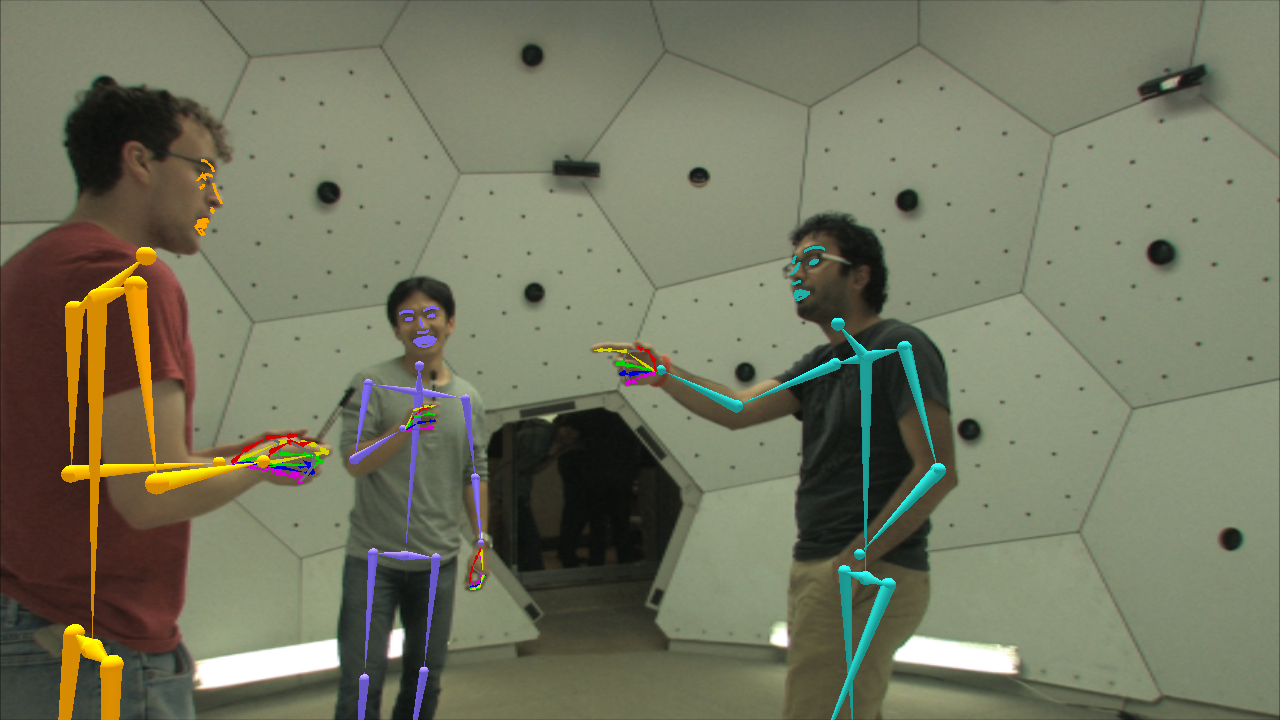
\includegraphics[width=0.24\columnwidth,trim=1000 110 1000 90, clip]{fig/totallinear/00000}
%	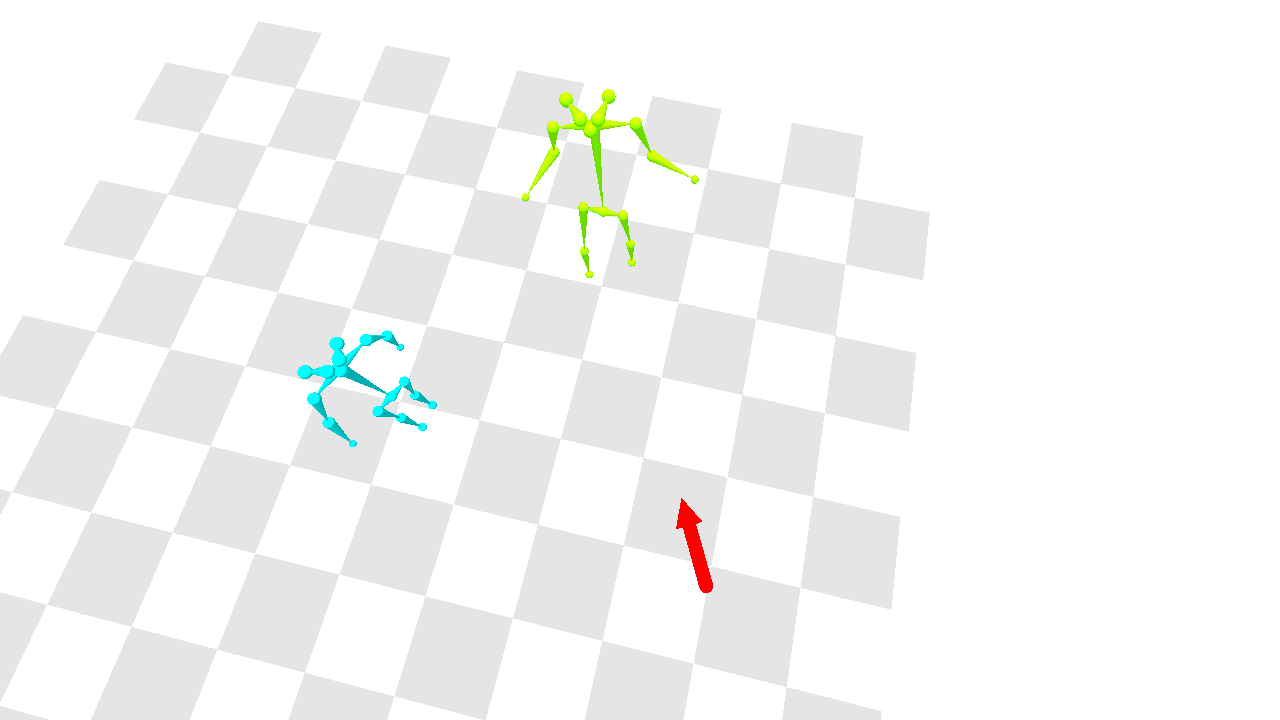
\includegraphics[width=0.24\columnwidth,trim=1000 110 1000 90, clip]{fig/totallinear/00001}	
%	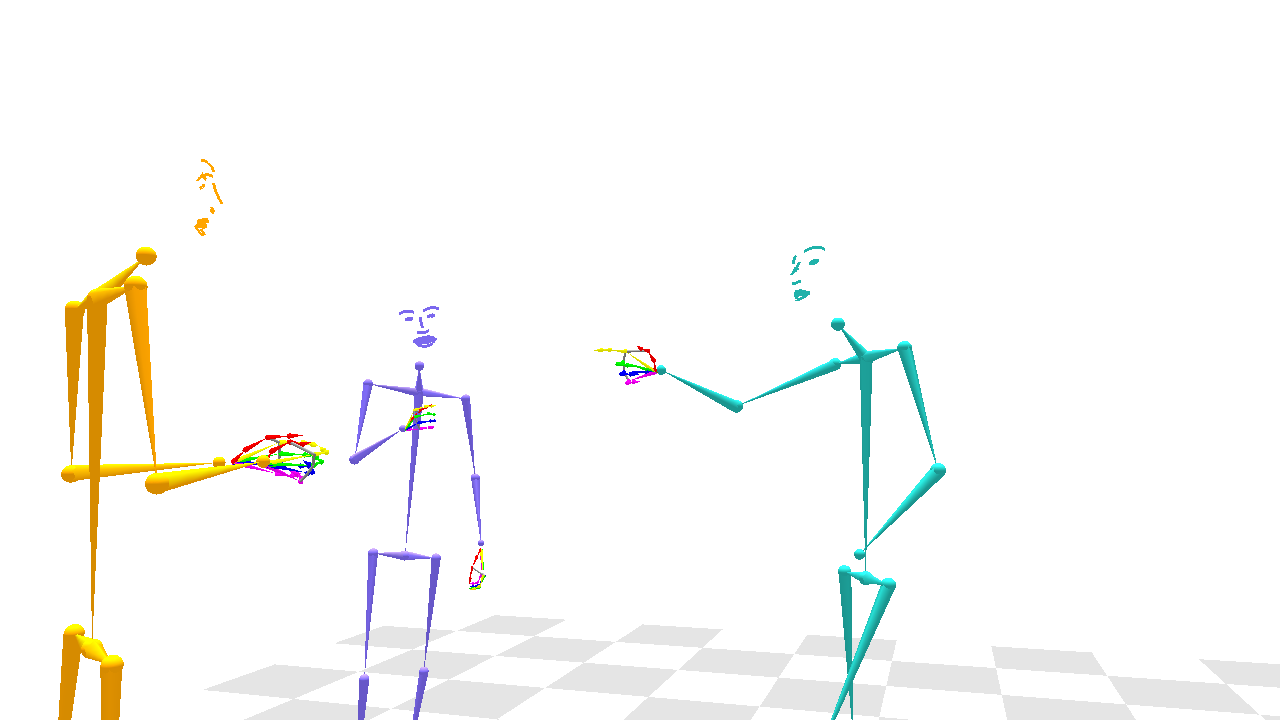
\includegraphics[width=0.24\columnwidth,trim=1000 110 1000 90, clip]{fig/totallinear/00002}
%	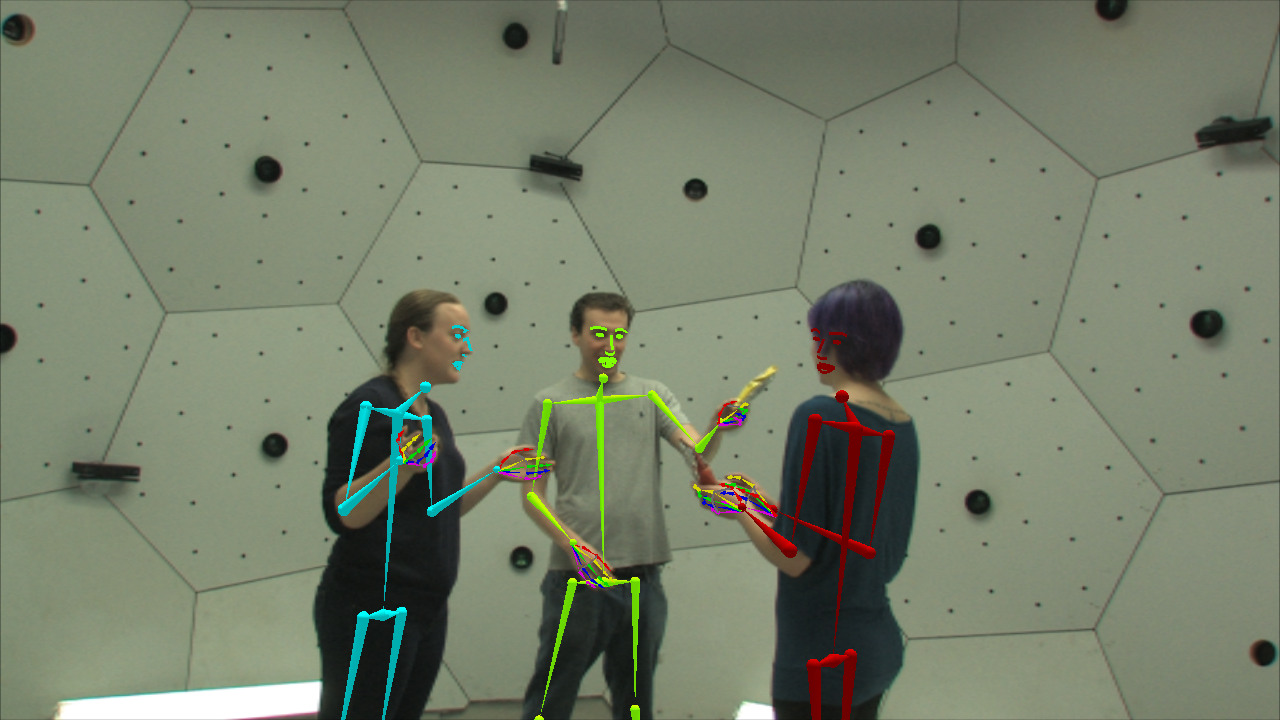
\includegraphics[width=0.24\columnwidth,trim=1000 110 1000 90, clip]{fig/totallinear/00003}	
%	\caption{Linear Blend Shapes for Total model. (a) mean shape; (b,c,d) after changing X-th,X-th,and X-th component respectively}
%	\label{fig:totallinearspace}
%\end{figure}
	
\subsection{Tracking with Adam}
% This section needs to be beefed up.
% Informal
The cost function to capture total body motion using Adam is similar to Eqn.~\ref{eq:fitting_franken} without the seam term:% ($E_\textrm{seam}$): 
\begin{align}
\label{eq:fitting_adam}
E\big( \boldsymbol{\theta}^A, \boldsymbol{\phi}^A, \boldsymbol{t}^A\big) = E_\textrm{keypoints} + E_\textrm{icp} +E_\textrm{prior}.
\end{align}
However, Adam is much more amenable to optimization than Frank: it has a single set of unified shape and pose parameters for all parts, and does not require seam constraints between disparate models. 
% Too informal

% The biggest advantage is setting the ratio among terms. E.g., seam term is tricky compared to others. 


%Conceptually, it is based on the SMPL model parameterization~\cite{Loper2015}, but with additional joints for the hands and facial expression blendshapes.

%\textbf{Optical Flow Propagation}: While fitting each frame independently has benefits----it does not suffer from error accumulation and frames can be fit in parallel---it typically produces jittery motion. To reduce this jitter, we use optical flow to propagate the initial, per-frame fit to neighboring frames to find a smoother solution. More concretely, given the fitting results at the frame $t$, we propagate this mesh to  frames $t{-}1$ and $t{+}1$ using optical flow at each vertex, which is triangulated into 3D using the method of~\cite{Joo2014}. Therefore, each vertex has at most three candidate positions: the original mesh, and the forward and backward propagated vertices (subject to a forward-backward consistency check). Given these propagated meshes, we reoptimize the model parameters by using all propagated mesh vertices as additional keypoints to find a compromise mesh. 
% In this case, every vertex has corresponding target locations by the propagated meshes. 
%We run this process multiple times (3, in our case), to further reduce jitter and fill in frames with missing detections.



% !TEX encoding = UTF-8 Unicode
% !TEX root = ../thesis.tex

\begin{figure}[t]	
%	\includegraphics[width=\columnwidth]{fig/quant/quant_visualization}
    \centering
	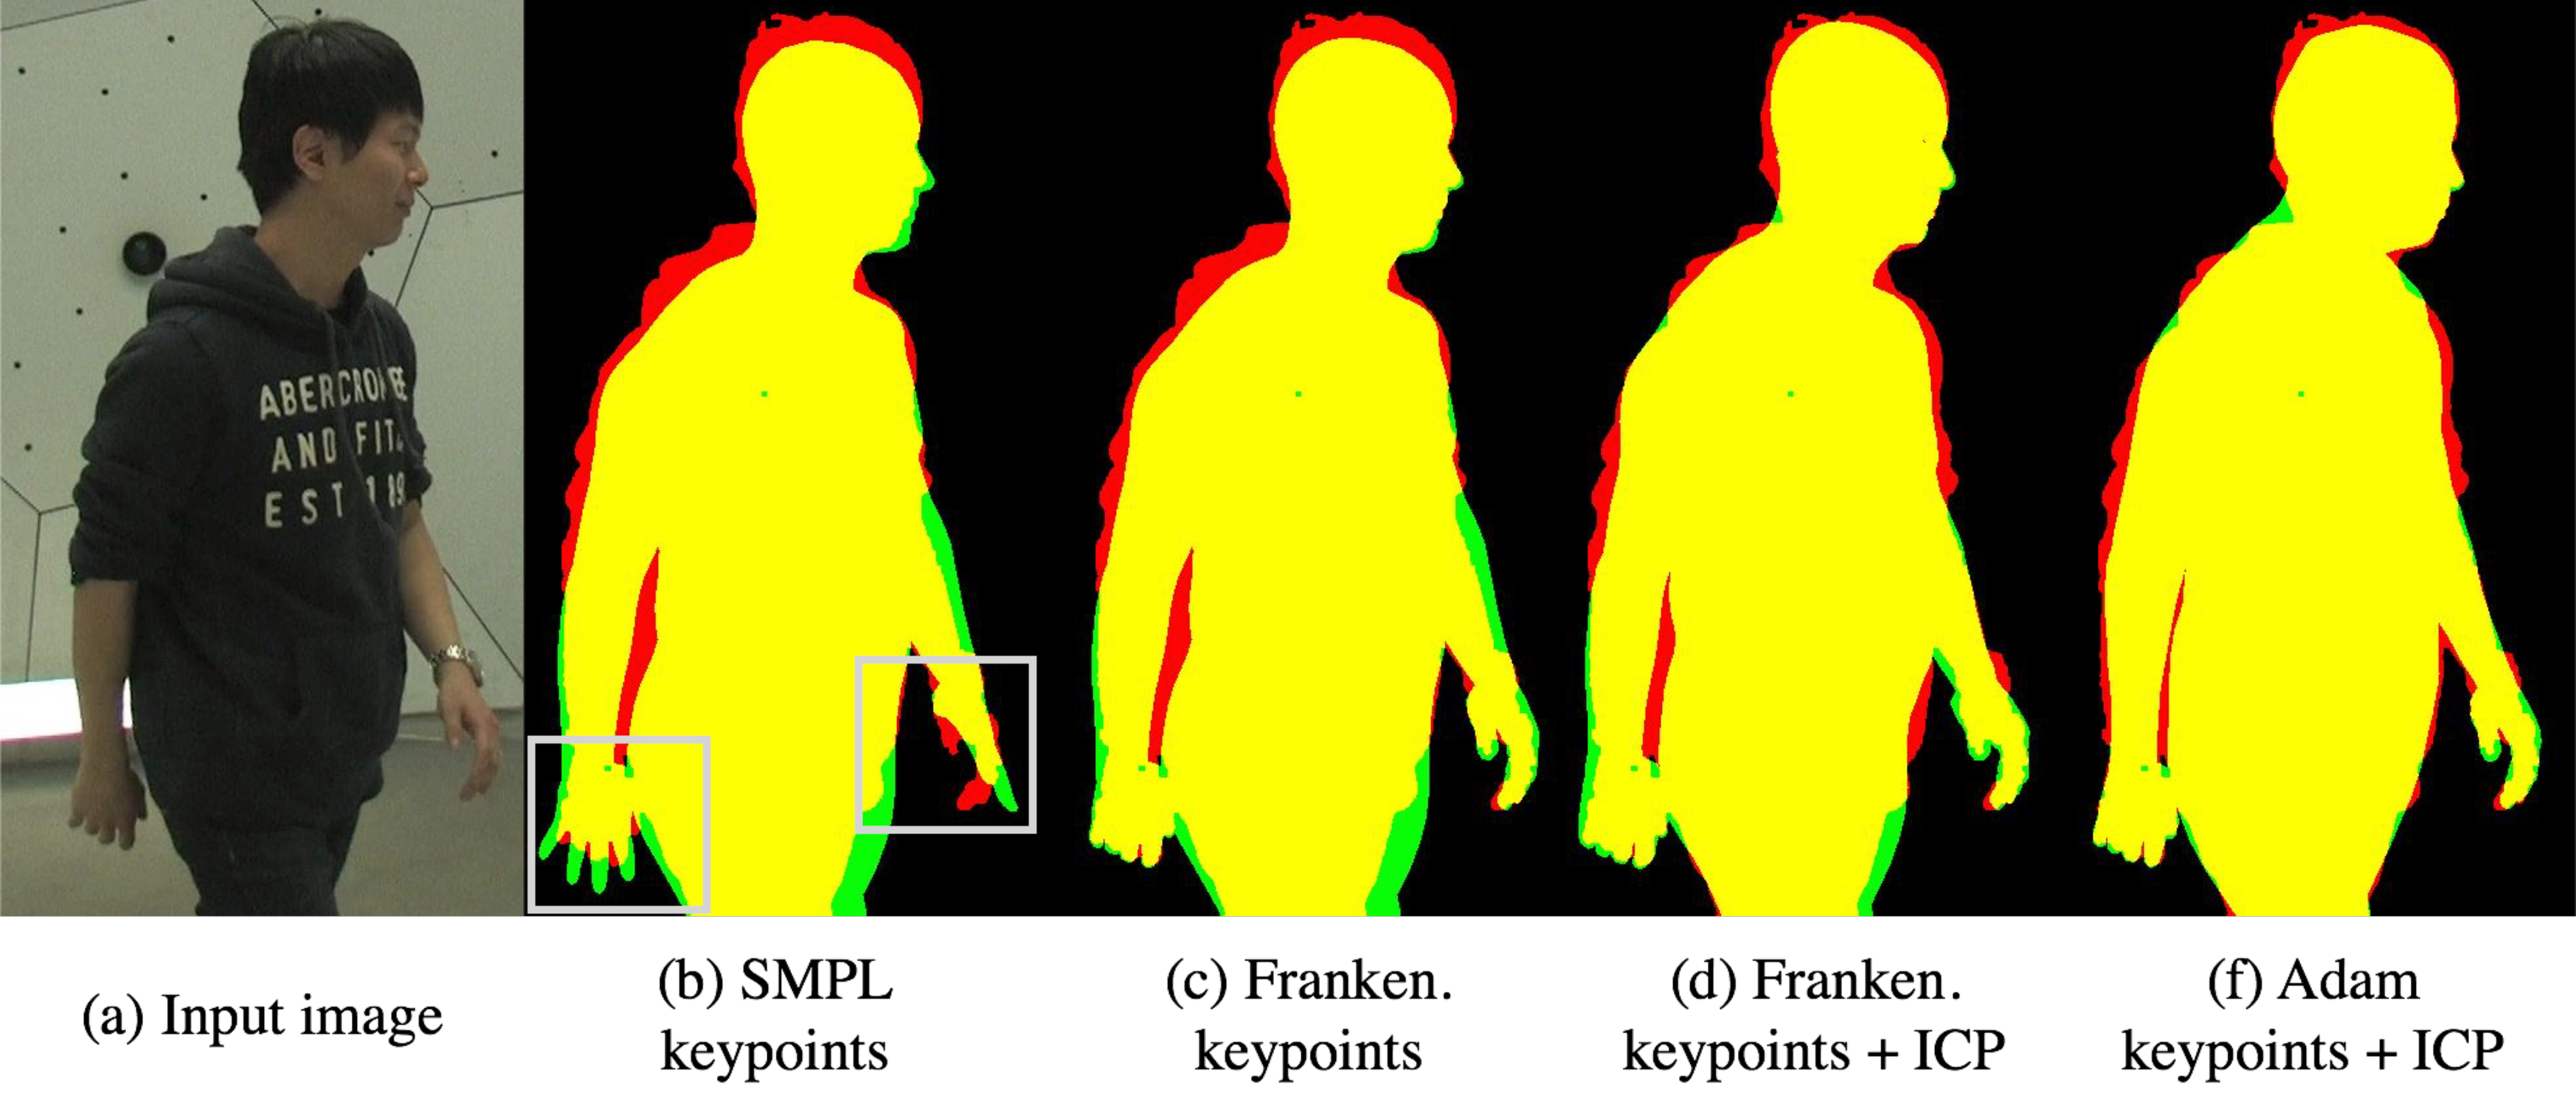
\includegraphics[width=0.9\columnwidth]{tbc_figures/quant_vis_legend}
	%\includegraphics[width=0.9\columnwidth]{fig/quant/silhoutte_quant_final_1115_2am}
	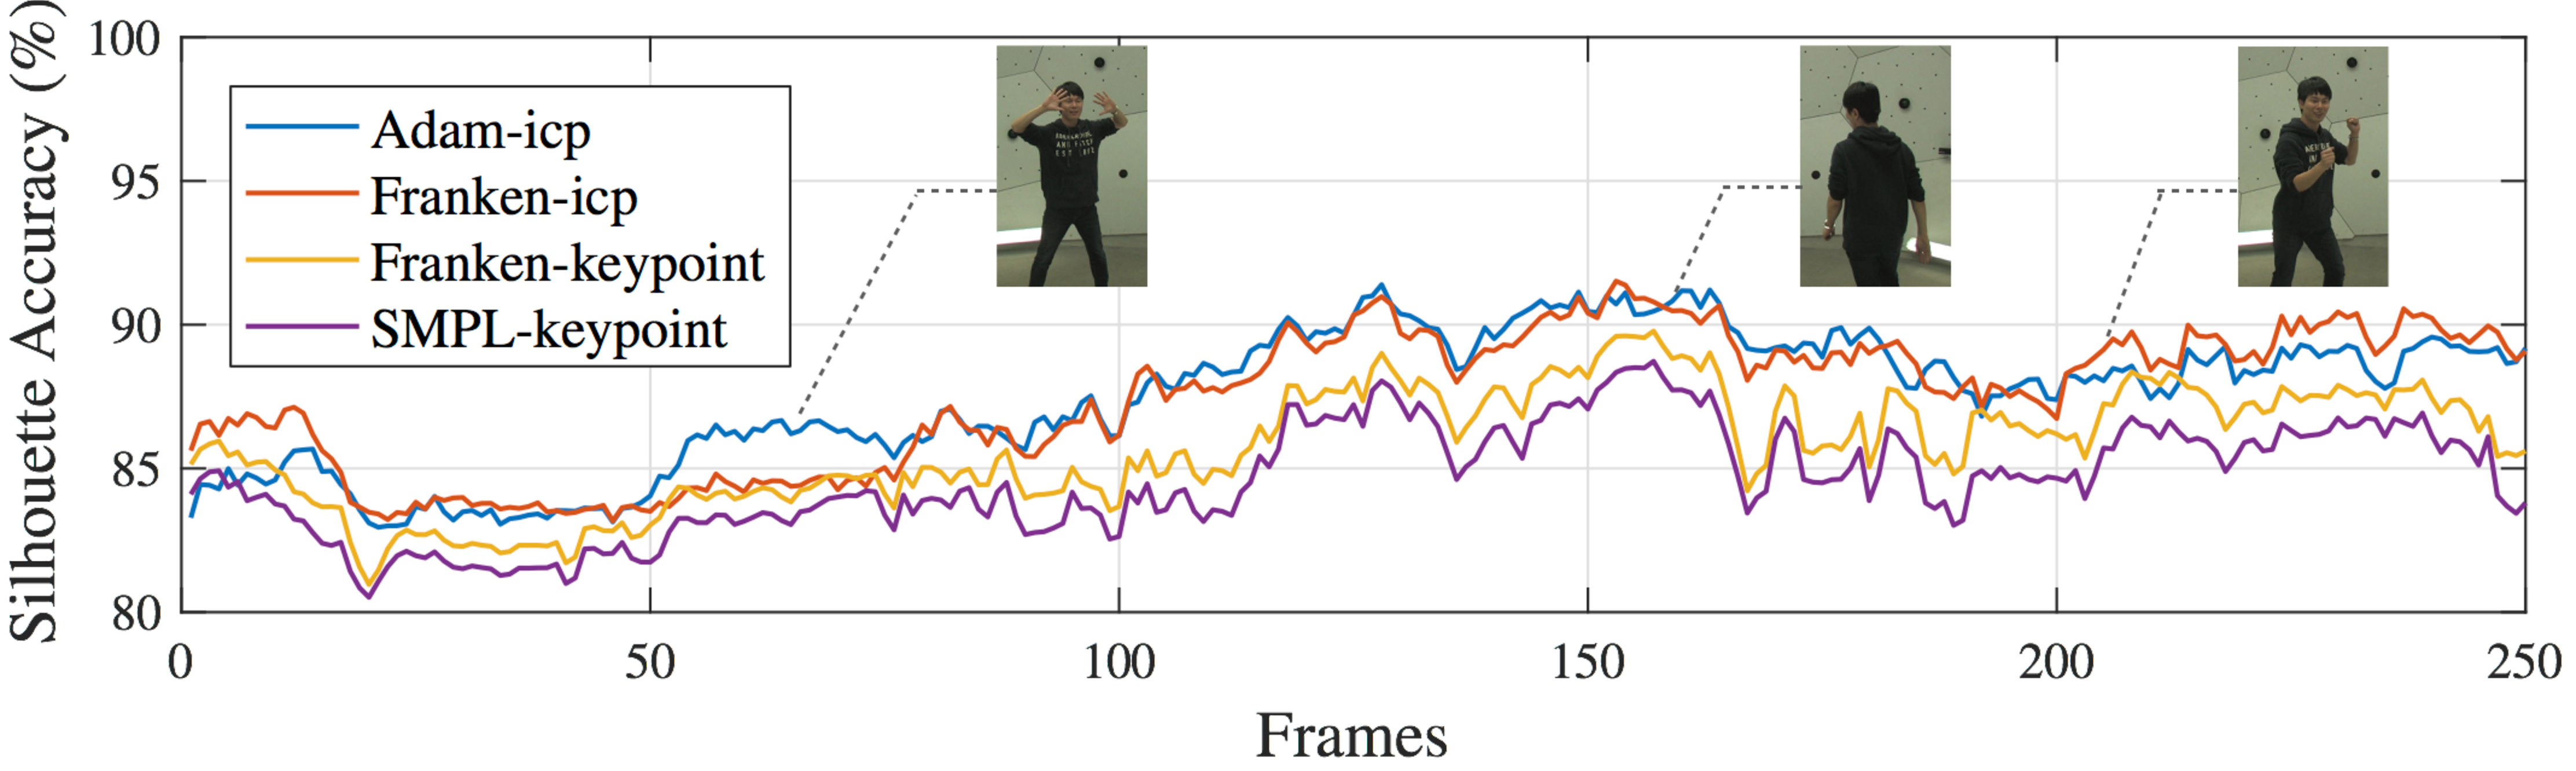
\includegraphics[width=0.9\columnwidth]{tbc_figures/quant_withFigures}
	\caption{(Top) The silhouette from different methods overlayed with ground-truth. The ground truth is drawn in the red channel and the rendered silhouette masks from each model are drawn in the green channel. Thus, the correctly overlapped region is shown as yellow color. (Bottom) Silhouette accuracy compared to the ground truth silhouette.}
	\label{fig:quant_silhoutte_vis}
\end{figure}

\begin{table} [t]	
\centering
\scriptsize
	\caption{Accuracy of Silhouettes from different models}\label{Table:quant_silhoette}
	\begin{tabular}{c|c|c|c|c}
		\hline 
		& {SMPL\cite{Loper2015}} & {Frank} & {Frank ICP} & {Adam ICP} \tabularnewline
		\hline 
		Mean &  84.79\% & 85.91\% & 87.68\% & 87.74\%  \tabularnewline
		\hline 
		Std.  &  4.55  & 4.57 & 4.53  & 4.18  \tabularnewline
		\hline 
	\end{tabular} 
	\label{table:quant_sillouette}
\end{table}

% \begin{figure}[t]
% 	\includegraphics[width=\columnwidth]{fig/quant/silhoutte_quant_final_1115_2am}
% 	\caption{Silhouette accuracy by the method of each model compared to the ground truth silhouette.}
% 	\label{fig:quant_silhoutte}
% \end{figure}

% Zoom into hands and faces

\begin{figure*}[t]
	%\includegraphics[width=\textwidth]{qualitativeResults3}
	%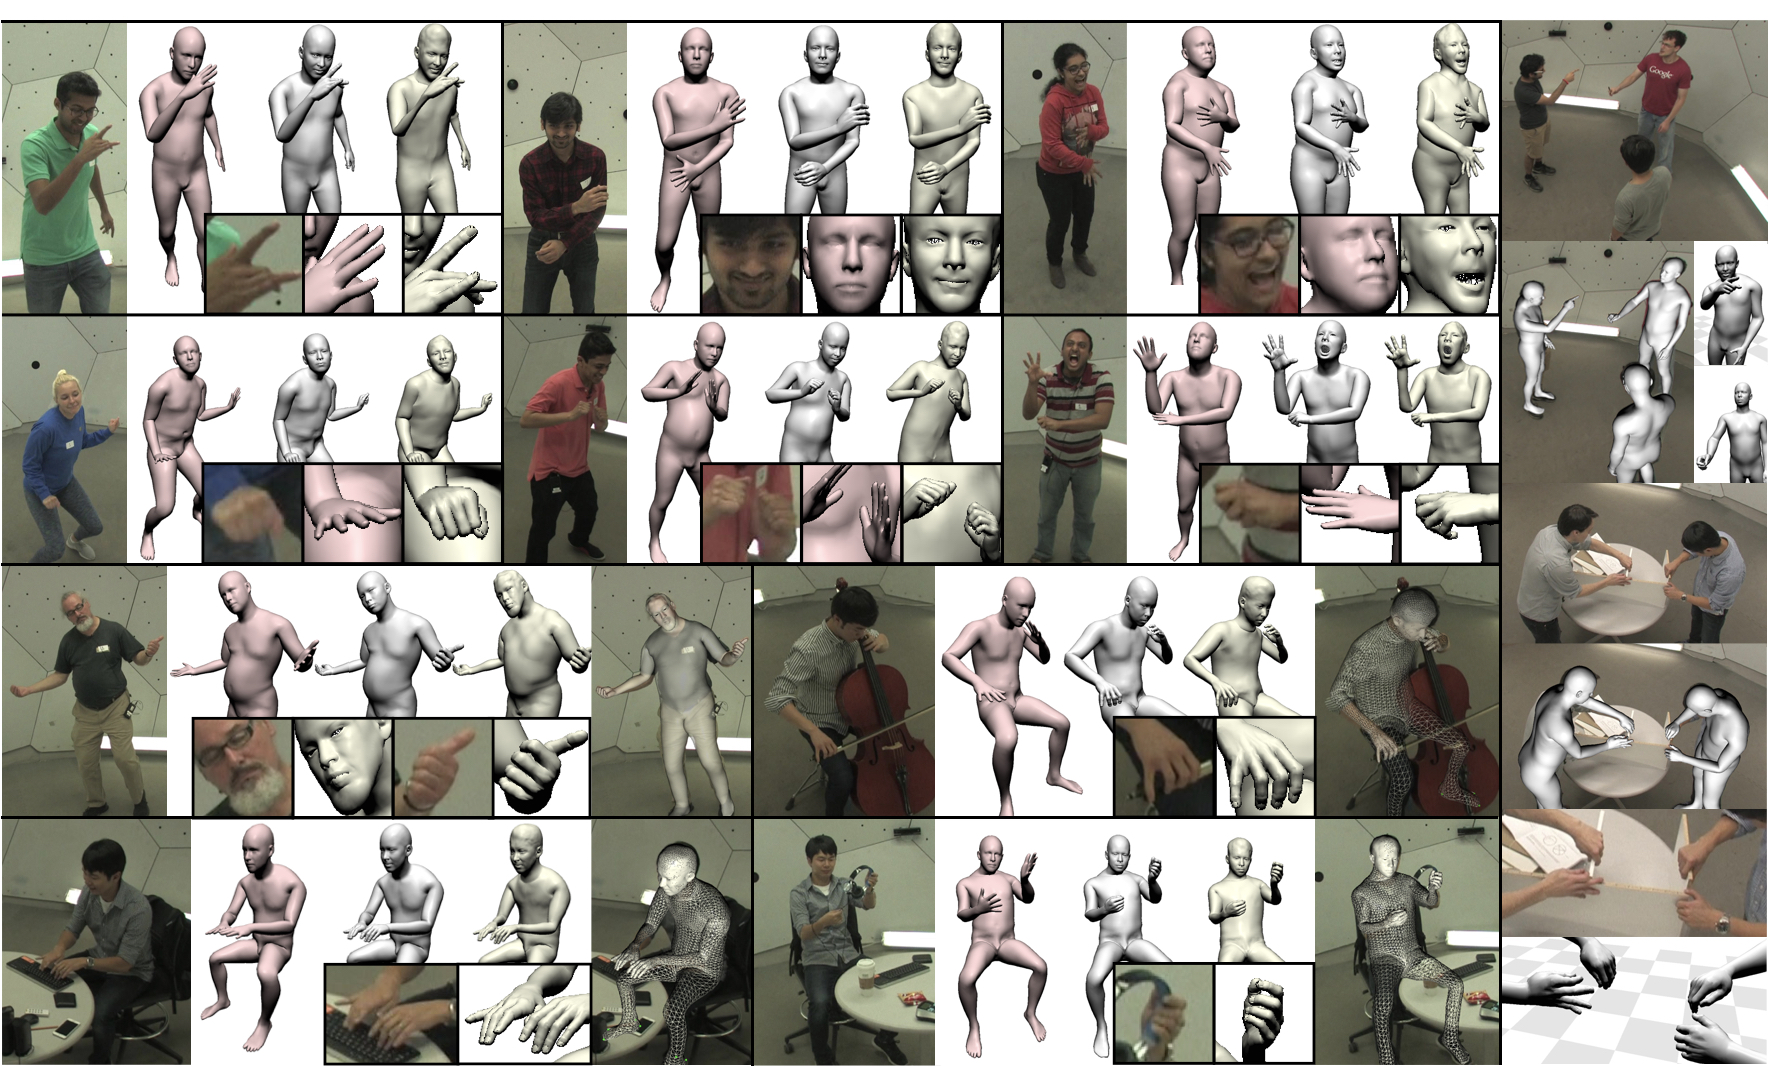
\includegraphics[width=\textwidth]{tbc_figures/Qualitative_180325.jpg}
	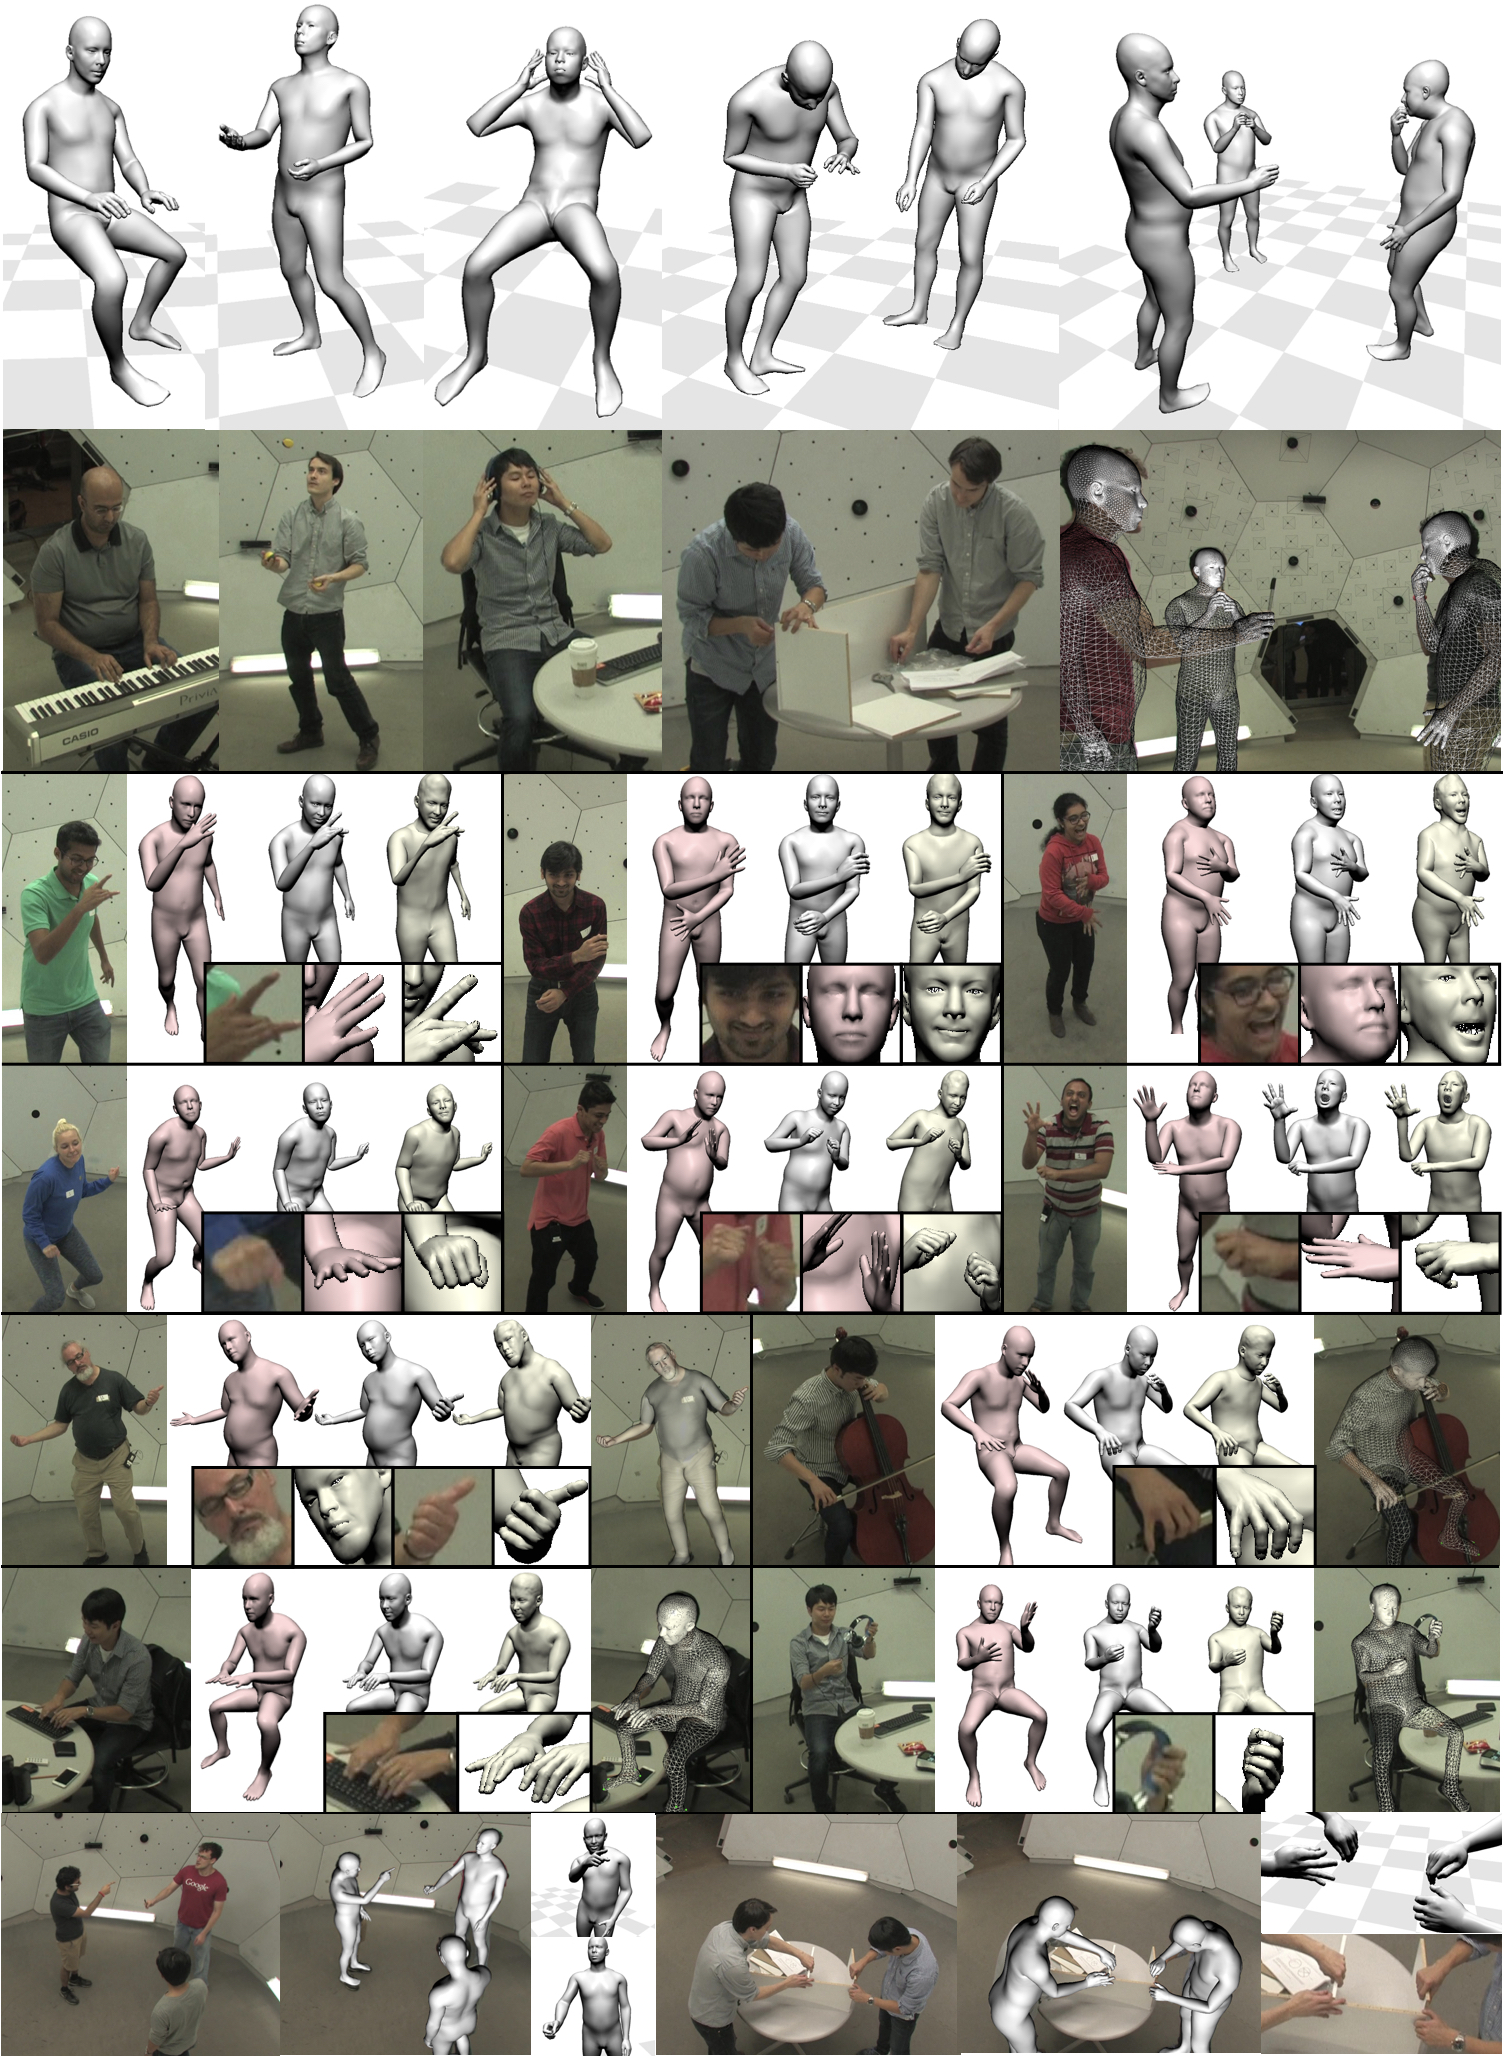
\includegraphics[width=\textwidth]{tbc_figures/Qualitative_thesis.jpg}
	\caption{Total body reconstruction results on various human body motions. For each example scene, the fitting results from three different models are shown by different colors (pink for SMPL~\cite{Loper2015}, silver for Frank, and gold for Adam). 
	%Facial expression and finger gestures captured by our two models provide more realism on the reconstruction output. The Adam model produces more subject-like outputs with simpler parameterization compared to the Frankenstein model.
	}
	\label{fig:qualitativeResults}
\end{figure*}
%

\section{Results}
We perform total motion capture using our two models, Frank and Adam, on various challenging sequences. For experiments, we use the dataset captured in the CMU Panoptic Studio~\cite{Joo-15, joo2017panoptic}. We use 140 VGA cameras to reconstruct 3D body keypoints, 480 VGA cameras for feet, and 31 HD cameras for faces and hands keypoints, and 3D point clouds. We compare the fits produced by our models with the simplified\footnote{In all our comparison, we disabled the pose-dependent blendshapes of SMPL, and thus here SMPL model means the body part of Frank.} SMPL model~\cite{Loper2015}. %In our evaluation, all reconstructions are performed per-frame independently. 

\subsection{Quantitative Evaluation}
% There is no straightforward way to generate ground truth data for total body motion. Thus, we alternatively use ground truth silhouettes in each view as a way to quantify the performance of our method. Since we restrict models in their parameterization space only, this experiment can be considered as a way to quantify the expressive power of each models. To be more reliable, we use silhouettes from 5 different view points. 
We evaluate how well each model can match a moving person by measuring overlap with the ground truth silhouette across 5 different viewpoints for a 10 second sequence. To obtain the ground truth silhouette, we run a background subtraction algorithm using a Gaussian model for the color of each pixel, with post-processing by morphological transforms to remove noise. As an evaluation metric, we compute the percentage of overlap compared to the union between the GT silhouettes and the rendered forground masks after fitting each model. Here, we compare the fitting results of 3 different models: SMPL, our Frank, and our Adam models. The results are shown in Fig.~\ref{fig:quant_silhoutte_vis} and Table~\ref{table:quant_sillouette}. We first compare accuracy between SMPL and Frank model by using only 3D keypoints as measurement cues. The major source of improvement of Frank over SMPL is in the articulated hand model (by construction, the body is almost identical). Including ICP term as cues provides better accuracy. Finally in the comparison between our two models, they show almost similar performance. Ideally we expect Adam to outperform Frank because it has more expressive power for hair and clothing, and it shows better performance for certain body shapes (frame 50-75 in Fig.~\ref{fig:quant_silhoutte_vis}). However, Adam sometimes produces artifacts showing lower accuracy: it tends to generate thinner legs, mainly due to poor 3D point cloud reconstructions in the training data\footnote{Due to dark clothing combined with fewer camera views of the legs.}. However, Adam is simpler for total body motion capture and has potential to be improved once a large dataset is available with a more optimized capture setup.

% \begin{align}
% \frac{\hat{S}_{f}^c\cap S_{f}^c}{\hat{S}_{f}^c \cup S_{f}^c} 
% \label{eq:metric1}
% \end{align}
% where $\hat{S}_{f}^c$ and $S_{f}^c$ are ground truth and rendered silhouettes at frame $f$ and camera $c$. 

%Note that this evaluation is a necessary but not a sufficient condition, because it cannot 
%affected by both shape and motion discrepancy. And it is a necessary condition, not sufficient, because model can be arbitrary deformed or drift inside silhouette.  

%\begin{figure*}[t]
%	\includegraphics[width=\textwidth]{fig/qualitative_group}
%	\caption{Qualitative Results. For each row, (1) an example view; (2) Fitting by only SMPL model; (2) Fitting with Frankenstein model; (3) Fitting with Total model; (4) Other 3D views of the Total model reconstruction.}
%	\label{fig:qualitativeResults_group}
%\end{figure*}

\subsection{Qualitative Results}
We run our method on sequences where face and hand motions naturally occur. The sequences include short range of motion for 70 people used to build Adam, social interactions of multiple people, a furniture building sequence with dexterous hand motions, musical performances (cello and guitars), and commonly observable daily motions such as typing. Most of these sequences are rarely demonstrated in previous markerless motion capture methods since capturing subtle details is key to achieve realism.  Example results are shown in Figure~\ref{fig:qualitativeResults} but are best seen in the accompanying videos. Here, we also qualitatively compare our models (in silver color for Frank, and gold for Adam) with SMPL (without pose-blendshapes, in pink)~\cite{Loper2015}. Note that total body motion capture based on our models produces more realism by capturing subtle details from the hands and faces.




% Here, discuss what the advantages are of Adam over Frank.

\section{Discussion}
We present the first markerless method to capture total body motion including facial expression, body motion from torso and limbs, and hand gestures at a distance. To achieve this result, we present two types of models, Frank and Adam, which can express motion in each of the parts. Our reconstruction results show compelling and realistic results, even when using only sparse 3D keypoint detections to drive the models.  As a current limitation of our system, Adam lacks expressive power in surface details due to the limited number of subjects in training. However, the major value of Adam model over Frank lies in its simpler representation to capture total body motion, which can be useful for other applications.
%demonstrating that capturing all body parts are important due to their correlations. 

There are two interesting points our paper raises. First, markerless hand motion capture, often considered too challenging compared to body and face captures, shows better localization quality in our results. Body joints are located inside the body and are hard to localize for clothed subjects, and the accuracy of face reconstruction greatly decreases once the face is not facing any camera. However, hands are often bare and the hand keypoint detector~\cite{simon2017hand} provides guessed measurements with high confidence even in self-occlusions, which can be fused in multiple views. Second, our results show a potential that markerless motion capture can eventually outperform its marker-based counterpart. Marker-based methods strongly suffer from occlusions, making it hard to capture both body and hands together, while our method can still exploit measurements for occluded parts by learning-based keypoint detectors.
